\documentclass[11pt,a4paper]{article}
\usepackage[T1]{fontenc}
\usepackage[utf8]{inputenc}
\usepackage{lmodern}
\usepackage{mathpazo}
\usepackage[a4paper,margin=27mm,headheight=15pt]{geometry}
\usepackage{microtype,amsmath,amssymb,amsthm,mathtools,bm}
\usepackage{booktabs,longtable,array,graphicx,xcolor,enumitem}
\usepackage{fancyhdr}
\usepackage{xurl,needspace,placeins}
\usepackage[unicode,pdfencoding=auto]{hyperref}
\usepackage[nameinlink,capitalise]{cleveref}
\definecolor{ink}{HTML}{183653}
\definecolor{accent}{HTML}{246B77}
\definecolor{soft}{HTML}{EDF3F5}
\hypersetup{colorlinks=true,linkcolor=ink,citecolor=accent,urlcolor=accent,
  pdftitle={Boundary completion for quadratic polylogarithm feedback},
  pdfauthor={Research report prepared for the ProveIt project}}
\setlength{\emergencystretch}{2em}
\setlength{\parskip}{3pt}
\numberwithin{equation}{section}
\newtheorem{theorem}{Theorem}[section]
\newtheorem{proposition}[theorem]{Proposition}
\newtheorem{corollary}[theorem]{Corollary}
\newtheorem{lemma}[theorem]{Lemma}
\theoremstyle{definition}
\newtheorem{definition}[theorem]{Definition}
\newtheorem{remark}[theorem]{Remark}
\newcommand{\Li}{\operatorname{Li}}
\newcommand{\ee}{\mathrm e}
\newcommand{\ii}{\mathrm i}
\newcommand{\dd}{\mathrm d}
\newcommand{\C}{\mathbb C}
\newcommand{\R}{\mathbb R}
\newcommand{\N}{\mathbb N}
\newcommand{\Prob}{\mathbb P}
\newcommand{\E}{\mathbb E}
\newcommand{\coef}[2]{[#1^{#2}]}
\newcommand{\Uc}{U_{\mathrm c}}
\newcommand{\Rb}{R_{\mathrm b}}
\newcommand{\vc}{v_{\mathrm b}}
\newcommand{\ph}{\varphi}
\newcommand{\eps}{\varepsilon}
\newcommand{\Log}{\operatorname{Log}}
\newcommand{\rem}{\mathcal R}
\newcommand{\supp}{\operatorname{supp}}
\pagestyle{fancy}
\fancyhf{}
\fancyhead[L]{\small\color{ink}Quadratic polylogarithm feedback}
\fancyhead[R]{\small\color{ink}ProveIt research}
\fancyfoot[C]{\thepage}
\renewcommand{\headrulewidth}{0.3pt}
\setlist[enumerate]{itemsep=4pt,topsep=5pt}
\setlist[itemize]{itemsep=3pt,topsep=5pt}
\title{\color{ink}\bfseries Boundary Completion for\\Quadratic Polylogarithm Feedback\\[5pt]
  \large Convergent inverse transseries, logarithmic resonance,\\
  and coefficient transitions}
\author{Research report prepared for the ProveIt project}
\date{12 October 2026}
\begin{document}
\maketitle
\begin{abstract}
We resolve the boundary-feedback question explicitly left open in the
incoming report \emph{Resonant Polylogarithm Transseries}.  For the germ
$v(0)=0$ determined by
$uv-v^2/2=\Li_s(r\ee^v)$, we prove the exact Taylor radius, unique dominant
singularity, and leading coefficient law for every $s>0$ and $u>0$.
For $s>2$, the critical parameter is
$\Uc(s)^2=2\zeta(s)+\zeta(s-1)^2$.  Above it we prove the previously
conjectured $R^{-n}n^{-s}$ law, including all integer orders.  At equality
the three coefficient scales are $R^{-n}n^{-1-1/(s-1)}$ for $2<s<3$,
$R^{-n}n^{-3/2}(\log n)^{-1/2}$ for $s=3$, and $R^{-n}n^{-3/2}$ for
$s>3$, with explicit constants.  An exact integral normal form yields
convergent inverse charts in finitely many power and logarithmic
coordinates.  At order three an exact Lambert core gives every
inverse-logarithmic coefficient correction; the first correction has a
particularly simple constant.  We also construct a convergent uniform
chart as the order crosses three and prove the coefficient crossover
as the feedback parameter crosses its critical value.  The proofs use
classical polylogarithm continuation, holomorphic inversion, singularity
analysis, and a directly proved lattice local limit argument.  The
contribution is the completed nonlinear model, its exact constants and
charts, and the resolution of a repository conjecture; the general
stable-law and singularity-analysis mechanisms are credited to their
antecedents.  Reproducible algebraic and numerical checks accompany the
proofs.
\end{abstract}
\clearpage
\tableofcontents
\newpage
\section{Research question, source audit, and precise contribution}
\label{sec:scope}

The nonlinear feedback equation
\begin{equation}\label{eq:model}
 uv(r)-\frac{v(r)^2}{2}=\Li_s\bigl(r\ee^{v(r)}\bigr),
 \qquad v(0)=0,\qquad s>0,\quad u>0,
\end{equation}
provides a concrete meeting point for polylogarithms and transseries.
The polylogarithm supplies a boundary singularity whose exponent changes
with $s$.  Nonlinear inversion may reach that singularity before, after,
or exactly when the ordinary inverse derivative vanishes.  The equality
case produces fractional powers, logarithms, and iterated logarithms;
it is especially well suited to a precise distinction between a formal
expansion and a convergent analytic chart.

The source report \cite{RepoFeedback}, Theorem \texttt{thm:feedback},
proves the case in which an interior characteristic point exists.
Its first question in Section \texttt{sec:future} asks for the remaining
boundary cases and prints the supercritical coefficient constant as an
unproved candidate.  We prove that candidate and all critical cases.
This is a resolution of an explicitly stated project question, not a
claim to settle a previously established open problem in the wider
literature.

\subsection{Snapshot and comparison sources}

The repository was inspected at commit
\begin{center}
\small\texttt{6207c3d40047fd8d1400a4d509fee71c9a3a8132}.
\end{center}
The review covered the two topic indexes, the incoming-report index,
the five incoming ZIP articles, and the relevant critical-feedback
and endpoint articles in the Transseries collection.  It was a focused
mathematical audit, not a line-by-line verification of the complete
552-page Polylogarithms manuscript or of every Transseries report.
The source inventory and hashes are recorded in \texttt{provenance.json}.

\begin{longtable}{@{}>{\raggedright\arraybackslash}p{0.25\textwidth}>{\raggedright\arraybackslash}p{0.36\textwidth}>{\raggedright\arraybackslash}p{0.33\textwidth}@{}}
\toprule
Source & Result already available & Role in this report\\
\midrule
\endhead
Incoming feedback report \cite{RepoFeedback}
& Positive finite coefficients, exact interior radius and fold,
and the boundary conjecture
& Interior theorem credited; boundary conjecture proved and extended\\
Critical Hahn report \cite{RepoHahn}
& Linear feedback with power tails, critical fractional inverses,
stable coefficient laws, coupling crossover
& General mechanism and comparison model\\
Gaussian endpoint report \cite{RepoGaussian}
& Uniform order crossover for eventually exact power tails,
Lambert coordinates and local limits
& Antecedent for the order--logarithm scaling\\
Other four incoming articles \cite{RepoJets,RepoUniform,RepoNormalized,RepoFolds}
& Resonant order jets, ordinary polylogarithm inverse charts,
complex critical values and folds
& Prevents presenting those existing charts as new results\\
\bottomrule
\end{longtable}
\addtocounter{table}{-1}% This uncaptioned comparison is not a numbered table.

The nonlinear function arising here is
\begin{equation}\label{eq:fdef-intro}
 f_u(t)=u-\sqrt{u^2-2\Li_s(t)}.
\end{equation}
Even when its coefficients have a power-law tail, they are not in
general eventually an exact multiple of $n^{-s}$.  Thus the existing
theorems for a polylogarithm plus a finite polynomial do not by
themselves verify this model's endpoint continuation or its correction
constants.  We give those proofs explicitly.

\subsection{Classical inputs and novelty boundary}

We use the classical convergent Jonqui\`ere expansion
\begin{equation}\label{eq:jonquiere}
 \Li_s(\ee^{-x})=
 \Gamma(1-s)x^{s-1}+
 \sum_{k\ge0}\zeta(s-k)\frac{(-x)^k}{k!},
 \qquad 0<|x|<2\pi,
\end{equation}
for nonintegral positive $s$, with a fixed branch of $\Log x$.
At positive integers the colliding Gamma and zeta terms are combined
before the parameter limit is taken.  These are classical identities,
recorded in DLMF \S25.12 \cite{DLMFPolylog}.
All displayed local series below are restricted to sufficiently small
sectors within this convergence domain.

The conversion of local singular expansions into Taylor coefficient
asymptotics is the singularity-analysis theory of Flajolet and Odlyzko
\cite{FO}.  The relation between implicit generating functions,
conditioned sums, and stable laws is also classical; Janson
\cite{Janson}, especially Sections 17--18, provides an extensive
treatment.  We include the particular Fourier proof needed for a
varying feedback parameter, so that the uniformity is not left to an
unstated invocation of a fixed-distribution theorem.

The exact boundary formula, the nonlinear critical charts, the
order-three correction polynomials, and the explicit uniform order
chart are the results established here for \eqref{eq:model}.
Their novelty relative to the inspected repository is documented above.
A focused literature search found the standard general mechanisms and
their antecedents; it did not establish publication priority for every
model-specific formula.  No theorem is advertised as a new general
principle of probability or transseries.

\subsection{Conventions}

Write
\[
 a_n(s,u)=\coef r n v(r),\qquad
 A_s=\zeta(s-1)\quad(s>2),\qquad
 \Uc(s)=\sqrt{2\zeta(s)+A_s^2}.
\]
An assertion about the coefficients $a_n$ always concerns the germ
$v(0)=0$ of \eqref{eq:model}.  It is not automatically an assertion
about the ordinary compositional inverse of $-\Li_s(-\ee^x)$.
The incoming source already makes this distinction; the special
dilogarithm identification does not extend to arbitrary $s$.

All square roots on a positive real argument denote the positive root.
Local inverse branches are selected by positivity for positive real
variables and then continued to a slit sector.  A \emph{convergent
transseries chart} means a holomorphic function of finitely many small
coordinates whose ordinary multivariable Taylor series converges
absolutely after substitution.  This claim is stronger than a
Poincar\'e asymptotic expansion.  The asymptotic coefficient expansions
obtained after singularity transfer need not themselves converge.

\section{The complete radius and coefficient classification}
\label{sec:phase}

Here and below, an equivalent $a_n\sim C R^{-n}n^{-p}(\log n)^{-q}$
has a strictly positive constant $C$.  This is useful because it proves
that the specified point really is singular, in addition to describing
the coefficients.

\begin{theorem}[Complete feedback phase diagram]\label{thm:phase}
For every $s>0$ and $u>0$, \eqref{eq:model} has a unique holomorphic germ
at zero.  Every coefficient $a_n(s,u)$ is positive.  The following list
gives its exact Taylor radius and coefficient equivalent.  In every
case the positive radius is the unique singularity on the circle of
convergence, and the Taylor series converges absolutely on that circle.

\begin{enumerate}
\item If $0<s\le2$, or if $s>2$ and $u<\Uc(s)$, there is a unique
$t_*\in(0,1)$ such that
\begin{equation}\label{eq:characteristic}
 u^2=2\Li_s(t_*)+\Li_{s-1}(t_*)^2.
\end{equation}
With $w_* =\Li_{s-1}(t_*)$ and $R=t_*\ee^{w_*-u}$,
\begin{equation}\label{eq:interior-law}
 a_n\sim
 \sqrt{\frac{w_*}{2\pi(1+\Li_{s-2}(t_*))}}\,
 R^{-n}n^{-3/2}.
\end{equation}
This is the interior theorem of \cite{RepoFeedback}.

\item Suppose $s>2$ and $u>\Uc(s)$.  Define
\begin{equation}\label{eq:boundary-parameters}
 A=\zeta(s-1),\quad b=\sqrt{u^2-2\zeta(s)},\quad
 \vc=u-b,\quad \Rb=\ee^{-\vc}.
\end{equation}
Then $b>A$, the radius is $\Rb$, and
\begin{equation}\label{eq:supercritical-law}
 \boxed{\displaystyle
 a_n\sim \frac{b^{s-1}}{(b-A)^s}\,\Rb^{-n}n^{-s}.}
\end{equation}
This proves the candidate in the incoming source's first research
question, including every integral $s\ge3$.

\item Suppose $u=\Uc(s)$, $s>2$, so that $b=A$ in
\eqref{eq:boundary-parameters}.  The radius is again $\Rb$.  If
$2<s<3$, put $\alpha=s-1$ and $\rho=1/\alpha$.  Then
\begin{equation}\label{eq:critical-stable}
 a_n\sim
 \frac{(A/\Gamma(-\alpha))^{1/\alpha}}{-\Gamma(-1/\alpha)}
 \,\Rb^{-n}n^{-1-1/\alpha}.
\end{equation}
At $s=3$, with $A=\zeta(2)$,
\begin{equation}\label{eq:critical-log}
 a_n\sim\sqrt{\frac A\pi}\,
 \Rb^{-n}n^{-3/2}(\log n)^{-1/2}.
\end{equation}
If $s>3$, then
\begin{equation}\label{eq:critical-gaussian}
 a_n\sim
 \sqrt{\frac{A}{2\pi(1+\zeta(s-2))}}\,
 \Rb^{-n}n^{-3/2}.
\end{equation}
\end{enumerate}
\end{theorem}

The transition has two independent parameters.  Changing $u$ determines
whether the first obstruction is an interior fold or the endpoint
$t=1$.  Once the endpoint and the fold coincide, changing $s$ determines
the regularity of the endpoint.  In particular, the vanishing limit of
the finite-curvature constant as $s\downarrow3$ does not describe the
$s=3$ law: the logarithm changes the scale.

\subsection{Positivity and the positive real branch}

\begin{lemma}[Positive germ and parametrization]\label{lem:positive}
The unique germ of \eqref{eq:model} has $a_n\ge1/(un^s)>0$.
On the increasing part of the positive real branch it is parametrized by
\begin{equation}\label{eq:parametrization}
 f_u(t)=u-\sqrt{u^2-2\Li_s(t)},\qquad
 v=f_u(t),\qquad r=t\ee^{-f_u(t)}.
\end{equation}
The first stationary point of $r(t)$, when it exists, is exactly
\eqref{eq:characteristic}.
\end{lemma}

\begin{proof}
Write
\[
 \Phi(r,v)=\frac{v^2}{2u}+\frac1u\sum_{n\ge1}\frac{r^n\ee^{nv}}{n^s}.
\]
The implicit function theorem applies to $v=\Phi(r,v)$ at $(0,0)$,
because $\Phi_v(0,0)=0$.  Starting with zero and iterating $\Phi$
formally produces nonnegative coefficients.  If two zero-constant-term
series agree through degree $N-1$, their images agree through degree
$N$, so every coefficient stabilizes after finitely many iterations.
The direct term $r^n/(un^s)$ proves the strict lower bound.

Solving the quadratic at $v=0,t=0$ selects \eqref{eq:parametrization}.
Where its square root is positive,
\begin{equation}\label{eq:radius-derivative}
 \frac{\dd}{\dd t}\log r(t)=\frac1t
 \left(1-\frac{\Li_{s-1}(t)}{\sqrt{u^2-2\Li_s(t)}}\right).
\end{equation}
The function $2\Li_s(t)+\Li_{s-1}(t)^2$ is strictly increasing on
$(0,1)$.  Its limit is infinite for $s\le2$ and equals $\Uc(s)^2$
for $s>2$.  At an interior stationary point the radicand is
$\Li_{s-1}(t)^2>0$, so the stationary point occurs before a possible
zero of the radicand.  These facts prove all assertions.
\end{proof}

\subsection{Global convergence and absence of competing singularities}

We supply the details for $u\ge\Uc(s)$, the previously unproved
range.  The interior proof uses the same argument with $t_*$ in
place of $1$.

For $u\ge\Uc(s)$ the radicand is positive on $[0,1]$, and
\eqref{eq:radius-derivative} is positive for $0<t<1$.
The parametrized solution therefore increases from $(0,0)$ to
$(\Rb,\vc)$.  Fix $0\le r<\Rb$.  The real iterates of $\Phi(r,\cdot)$
starting at zero are bounded above by this solution.  Monotone
convergence, first in the iteration and then in the coefficient
index, shows that the formal series converges at this $r$.
Thus its radius is at least $\Rb$.  Its sum agrees with the
parametrized branch by local uniqueness and continuation.  Taking
$r\uparrow\Rb$ gives
\begin{equation}\label{eq:boundary-sum}
 \sum_{n\ge1}a_n\Rb^n=\vc<\infty.
\end{equation}
Consequently the series converges absolutely and uniformly throughout
the closed disk $|r|\le\Rb$.

Let $|r|=\Rb$, $r\ne\Rb$.  Strict positivity of every $a_n$ gives
$|v(r)|<\vc$: equality in the triangle inequality would force
$r^n/\Rb^n$ to have the same argument for every positive integer $n$.
It follows that
\[
 |r\ee^{v(r)}|<\Rb\ee^{\vc}=1.
\]
The defining equation is analytic at this boundary point, and
\begin{equation}\label{eq:boundary-derivative}
 |\Phi_v(r,v(r))|
 \le\frac{|v(r)|+\Li_{s-1}(|r\ee^{v(r)}|)}u
 <\frac{\vc+A}{u}\le1.
\end{equation}
The implicit function theorem extends the germ across every such
point.  Therefore $\Rb$ is the only possible singularity on the
circle.  The local singular expansions below prove that it is
indeed singular and hence that the radius is exactly $\Rb$.

\subsection{An exact integral normal form}

Define, for $s>2$ and $x$ in a small slit neighborhood of zero,
\begin{equation}\label{eq:DK}
 D_s(x)=\zeta(s)-\Li_s(\ee^{-x}),\qquad
 K_s(x)=A x+\frac{x^2}{2}-D_s(x).
\end{equation}
Since $D_s'(x)=\Li_{s-1}(\ee^{-x})$,
\begin{equation}\label{eq:K-integral}
 \boxed{\displaystyle
 K_s(x)=\int_0^x(x-t)\bigl(1+\Li_{s-2}(\ee^{-t})\bigr)\,\dd t.}
\end{equation}
The integral is along the radial segment on the chosen branch.
It converges at zero for $s>2$, including $2<s\le3$.
Indeed the singular part of its integrand is of order
$t^{s-3}$ or $\log t$, and $s-3>-1$.

Put $x=-\Log t$ and $d=-\Log(r/\Rb)$.  The parametrization gives
the exact equations
\begin{align}
 d&=\Psi_b(x):=x+b-\sqrt{b^2+2D_s(x)},\label{eq:Psi}\\
 v(r)&=\vc+d-x,\label{eq:v-x}\\
 (b+x)d-\frac{d^2}{2}&=(b-A)x+K_s(x).\label{eq:normalform}
\end{align}
The last identity follows by squaring the first one, using the root
that tends to $b$.  Conversely, near zero, that root condition recovers
\eqref{eq:Psi}; no extra local inverse branch is introduced by the
squaring.  At the critical parameter the linear term disappears:
\begin{equation}\label{eq:critical-normalform}
 \boxed{\displaystyle K_s(x)=(A+x)d-\frac{d^2}{2}.}
\end{equation}
This single equation is the starting point of all the convergent
critical charts below.

\subsection{The local singularities}

For nonintegral $s>2$, set $\alpha=s-1$.  Equation
\eqref{eq:jonquiere} gives the convergent identity
\begin{equation}\label{eq:K-noninteger}
 K_s(x)=\Gamma(-\alpha)x^\alpha+x^2 B_s(x),\qquad
 B_s(x)=\frac{1+\zeta(s-2)}2+
 \sum_{k\ge3}\zeta(s-k)\frac{(-1)^k x^{k-2}}{k!}.
\end{equation}
For an integer $m\ge3$ the corresponding resonant formula is
\begin{equation}\label{eq:K-integer}
 K_m(x)=\frac{x^2}{2}
 +\sum_{\substack{k\ge2\\k\ne m-1}}
   \zeta(m-k)\frac{(-x)^k}{k!}
 +\frac{(-x)^{m-1}}{(m-1)!}
   \bigl(H_{m-1}-\Log x\bigr).
\end{equation}
The separate $x^2/2$ remains present when $m=3$.
In that case
\begin{equation}\label{eq:K3}
 K_3(x)=\frac{x^2}{2}\left(\log\frac1x+\frac52\right)
       +\frac{x^3}{12}-\frac{x^4}{288}+O(x^6).
\end{equation}
The absence of the $x^5$ term is $\zeta(-2)=0$.

At $b=A$, \eqref{eq:critical-normalform} now gives
\begin{equation}\label{eq:Psi-critical-leading}
 \Psi_A(x)\sim
 \begin{cases}
  \dfrac{\Gamma(1-s)}A x^{s-1},&2<s<3,\\[4pt]
  \dfrac{x^2}{2A}\log(1/x),&s=3,\\[4pt]
  \dfrac{1+\zeta(s-2)}{2A}x^2,&s>3.
 \end{cases}
\end{equation}
All equivalents hold uniformly on closed subsectors of the slit.
For $b>A$ the leading term is instead
$\Psi_b(x)\sim\kappa x$, where $\kappa=1-A/b>0$.

\begin{lemma}[Sectorial inverse and dented continuation]\label{lem:delta}
Each boundary branch above has a holomorphic inverse $x(d)$ in a
sufficiently small sector $|\arg d|<\pi-\eta$, for any fixed
$0<\eta<\pi$, selected by $x>0$ when $d>0$.  Together with
\eqref{eq:boundary-derivative}, this supplies a dented disk at
$r=\Rb$ of the type required for singularity transfer.
\end{lemma}

\begin{proof}
For $\Psi(x)\sim c x^p$, $c>0$, $p\ge1$, take
$x_0=(d/c)^{1/p}$.  On a small fixed relative circle
$|x/x_0-1|=\epsilon$, the normalized function $\Psi(x)/d-1$
converges uniformly to $(x/x_0)^p-1$, which has one simple zero
inside.  Rouch\'e's theorem gives a unique root near $x_0$.
The differentiated convergent expansions show that the derivative
is nonzero there.  The local implicit inverses glue by uniqueness.
For $\Psi(x)\sim c x^2\log(1/x)$, the same proof uses
$x_0=(2d/(c\log(1/d)))^{1/2}$; the slowly varying logarithm has
ratio tending to one on the relative circle.  These arguments
use the differentiated expansions, rather than differentiating an
arbitrary unspecified $o(1)$.

The variable $d=-\Log(r/\Rb)$ is analytic near $r=\Rb$ and equals
$1-r/\Rb+O((1-r/\Rb)^2)$.  Its slit sector supplies the local
dent.  The rest of the circle has analytic extensions by
\eqref{eq:boundary-derivative}.  A finite cover of its compact
arcs completes a dented disk after its thickness is decreased.
\end{proof}

\subsection{Proof of the coefficient laws}

For nonintegral $s>2$ and $b>A$, regard $x$ and $x^\alpha$ as
independent local coordinates.  In \eqref{eq:Psi}, the coefficient
of its first nonanalytic term is $\Gamma(-\alpha)/b$.
The inverse therefore has first nonanalytic term
\[
 -\frac{\Gamma(-\alpha)}{b\kappa^{\alpha+1}}d^\alpha.
\]
One way to verify the factor is to substitute the analytic inverse
$x_{\rm an}(d)=d/\kappa+O(d^2)$ and divide the perturbation by
$\Psi'_{\rm an}(0)=\kappa$.  Equation \eqref{eq:v-x} changes its
sign.  Thus the singular term of $v$ is
\begin{equation}\label{eq:super-singular}
 \frac{\Gamma(1-s)}{b\kappa^s}d^{s-1}.
\end{equation}
Transfer of $(1-z)^{s-1}$ divides by $\Gamma(1-s)$ and gives
\eqref{eq:supercritical-law}.

The integer case can be checked directly, avoiding any interchange
of a parameter limit and a coefficient asymptotic.  For $s=m\ge3$,
put $j=m-1$.  The singular term of $v$ is
\begin{equation}\label{eq:integer-super-singular}
 \frac{(-1)^{j+1}}{b\,j!\,\kappa^m}d^j\Log d.
\end{equation}
The exact logarithmic transfer equivalent is
\[
 \coef z n (1-z)^j\Log(1-z)
 \sim(-1)^{j+1}j!\,n^{-j-1}.
\]
The signs and factorials cancel, giving the same positive constant
$1/(b\kappa^m)$.

At criticality, inversion of \eqref{eq:Psi-critical-leading} and
\eqref{eq:v-x} yields respectively
\begin{align*}
 v&=\vc-(A/\Gamma(-\alpha))^{1/\alpha}d^{1/\alpha}
       +o(d^{1/\alpha}),&&1<\alpha<2,\\
 v&=\vc-2\sqrt A\,d^{1/2}(\log(1/d))^{-1/2}
       \left(1+O\left(\frac{\log\log(1/d)}{\log(1/d)}\right)\right),
       &&s=3,\\
 v&=\vc-\sqrt{\frac{2A}{1+\zeta(s-2)}}d^{1/2}
       +o(d^{1/2}),&&s>3.
\end{align*}
The term $d$ in \eqref{eq:v-x} is locally analytic and is smaller
than the displayed singular terms.  Apply \cref{lem:delta} and the
power--logarithm transfer theorem \cite{FO}.  Since
$\Gamma(-1/2)=-2\sqrt\pi$, this proves
\eqref{eq:critical-stable}--\eqref{eq:critical-gaussian}.
The local expansions prove genuine singularity and complete the
radius argument.  At an interior point the usual implicit quadratic
expansion has amplitude
$\sqrt{2w_* /(1+\Li_{s-2}(t_*))}$; the same transfer gives
\eqref{eq:interior-law}.  This also reproves the part credited to
the incoming report.

\begin{corollary}[The physical convergence threshold for every order]
\label{cor:physical}
For every $s>0$ there is a unique $t_s\in(0,1)$ satisfying
\begin{equation}\label{eq:physical-t}
 \log t_s+\Li_{s-1}(t_s)=0.
\end{equation}
Put $u_s^2=2\Li_s(t_s)+\Li_{s-1}(t_s)^2$.
The Taylor series of $v$ evaluated at $r=-\ee^{-u}$ converges if and
only if $u\ge u_s$.  At equality it converges absolutely.
\end{corollary}

\begin{proof}
The left side of \eqref{eq:physical-t} is strictly increasing from
$-\infty$ to a positive limit.  In the interior regime,
$\ee^{-u}/R=\ee^{-w_*}/t_*$, so the condition that the evaluation
point lie on or within the convergence circle is precisely
$\log t_*+w_*\ge0$.  Monotonicity of the characteristic equation
proves the stated threshold.  If $s>2$, then $u_s<\Uc(s)$.
For all $u\ge\Uc(s)$ the boundary radius instead satisfies
$\ee^{-u}/\Rb=\ee^{-b}<1$.  Absolute convergence at equality
follows from \cref{thm:phase}.
\end{proof}

The incoming report proves this last statement for $0<s\le2$.
The boundary classification removes that restriction.

\section{Convergent inverse charts at the critical endpoint}
\label{sec:charts}

We now resolve the critical singularity beyond its leading equivalent.
Throughout this section $u=\Uc(s)$, $s>2$, and the inverse is selected by
$x>0$ when $d>0$.  Its exact equation is
\eqref{eq:critical-normalform}.  All fractional powers are continued
from the positive axis in the sector supplied by \cref{lem:delta}.
A power of a function near $1$ uses the Taylor-series logarithm there.
Every chart below is holomorphic in finitely many independent small
coordinates; its convergent Taylor series becomes an exact generalized
power or logarithmic series after the indicated substitution.

\subsection{The range \texorpdfstring{$2<s<3$}{2<s<3}}

Put
\[
 \alpha=s-1,\qquad \beta=2-\alpha=3-s,\qquad
 C=\Gamma(1-s)>0,
\]
and use $B_s$ from \eqref{eq:K-noninteger}.  Thus
$K_s(x)=Cx^\alpha+x^2B_s(x)$.  Write
\[
 B_0=B_s(0)=\frac{1+\zeta(s-2)}2,\qquad
 B_1=B_s'(0)=-\frac{\zeta(s-3)}6.
\]
The two small exponents $\alpha-1$ and $\beta$ are both positive
and sum to one.  This relation removes the need for a third generator.

\begin{theorem}[A convergent chart with polynomial sectors]
\label{thm:chart-low}
Define
\begin{equation}\label{eq:chart-low-coordinates}
 q=\left(\frac{Ad}{C}\right)^{1/\alpha},\qquad
 p=q^{\alpha-1},\qquad z=q^\beta.
\end{equation}
There is a unique holomorphic germ $U(p,z)$ at $(0,0)$, with
$U(0,0)=1$, satisfying
\begin{equation}\label{eq:chart-low-equation}
 U^\alpha+\frac zC U^2 B_s(pzU)
 =1+\frac{pz}{A}U-\frac{C}{2A^2}p^2z.
\end{equation}
The critical inverse is exactly
\begin{equation}\label{eq:chart-low-inverse}
 x=qU(q^{\alpha-1},q^\beta).
\end{equation}
Moreover,
\begin{equation}\label{eq:chart-low-sectors}
 U(p,z)=1+\sum_{\ell\ge1}P_\ell(p)z^\ell,
 \qquad P_\ell\in\R[p],\qquad \deg P_\ell\le2\ell,
\end{equation}
with normal convergence on a sufficiently small bidisk.
\end{theorem}

\begin{proof}
Substitute $x=qU$ and $d=Cq^\alpha/A$ into
\eqref{eq:critical-normalform}, then divide by $Cq^\alpha$.
Since $q=pz$ and $q^\alpha=p^2z$, the result is
\eqref{eq:chart-low-equation}.  Its derivative in $U$ at
$(p,z,U)=(0,0,1)$ is $\alpha\ne0$.  The holomorphic implicit
function theorem gives the germ.  Substitution recovers the original
equation, and \cref{lem:delta} identifies the selected inverse.

At $z=0$ the solution is $U=1$.  In the perturbation side obtained
after isolating $U^\alpha-1$, every monomial $p^jz^\ell$ has
$\ell\ge1$ and $j\le2\ell$.  The three sources of such monomials
are $pz$, $p^2z$, and $p^jz^{j+1}$ from the analytic tail.
Induction on the $z$-degree in the implicit coefficient recursion
preserves this support condition.  It proves the polynomial assertion;
holomorphy proves convergence.
\end{proof}

There is a finite formula for every sector polynomial.  Put
\begin{align*}
 F_0(h)&=(1+h)^\alpha-1,\\
 \Psi(p,z,h)&=\frac{pz}{A}(1+h)-\frac{Cp^2z}{2A^2}
 -\frac zC(1+h)^2B_s(pz(1+h)).
\end{align*}
Then
\begin{equation}\label{eq:chart-low-finite}
 P_\ell(p)=\sum_{k=1}^{\ell}\frac1k
 [z^\ell h^{k-1}]
 \left\{\frac h{F_0(h)}\Psi(p,z,h)\right\}^{k}.
\end{equation}
Indeed, insert an auxiliary multiplier on $\Psi$ in $F_0(h)=\Psi$,
rewrite this as a Lagrange equation for $h$, and extract its coefficients.
Since $\Psi$ is divisible by $z$, only $k\le\ell$ can contribute.
This finite extraction agrees with the Taylor coefficients of the
already established analytic germ; no convergence assertion about the
auxiliary multiplier is needed.

For example,
\begin{align}
 P_1(p)&=-\frac{B_0}{\alpha C}+
          \frac p{\alpha A}-\frac{Cp^2}{2\alpha A^2},
          \label{eq:chart-low-P1}\\
 P_2(p)&=\frac1\alpha\left\{
 \left(\frac pA-\frac{2B_0}C\right)P_1(p)-\frac{B_1p}C
 -\frac{\alpha(\alpha-1)}2P_1(p)^2\right\}.
          \label{eq:chart-low-P2}
\end{align}
The whole ladder at $p=0$ has the closed form
\begin{equation}\label{eq:chart-low-pure}
 P_\ell(0)=
 \frac{(-B_0/C)^\ell}{\alpha\,\ell!}
 \frac{\Gamma((2\ell+1)/\alpha)}
 {\Gamma(1+(1+\ell\beta)/\alpha)}.
\end{equation}
To prove it, set $p=0$ in the chart and put $w=U^\alpha$.
The equation becomes $w+(B_0/C)zw^{2/\alpha}=1$;
ordinary Lagrange inversion applied to $w^{1/\alpha}$ gives
\eqref{eq:chart-low-pure}.

The terms of total Taylor degree at most two are
\begin{equation}\label{eq:chart-low-first}
 U=1-\frac{B_0}{\alpha C}z+\frac1{\alpha A}pz
 +\frac{(5-\alpha)B_0^2}{2\alpha^2C^2}z^2
 +O((|p|+|z|)^3).
\end{equation}
Their asymptotic order after substitution depends on $s$; equal powers
must be collected when the two exponents are rationally related.
In particular, if $B_0\ne0$,
\[
 x=q-\frac{B_0}{\alpha C}q^{1+\beta}+o(q^{1+\beta}).
\]
There is a genuine cancellation possibility.  If $\zeta(s-2)=-1$,
then $B_0=0$ and the entire ladder \eqref{eq:chart-low-pure} vanishes.
In this case $U(p,0)=U(0,z)=1$, so $U-1$ is divisible by $pz=q$.
Equation \eqref{eq:chart-low-P1} therefore gives instead
\begin{equation}\label{eq:chart-low-cancellation}
 x=q+\frac{q^2}{\alpha A}+o(q^2).
\end{equation}
No uniqueness claim about an order satisfying this cancellation condition
is needed for the result.

\subsection{An exact Lambert chart at order three}

Let $s=3$, $A=\zeta(2)$, and define the analytic tail $C_3$ by
\[
 K_3(x)=\frac{x^2}{2}\left(\log\frac1x+\frac52\right)+x^3C_3(x).
\]
By \eqref{eq:K3},
$C_3(x)=1/12-x/288+O(x^3)$; its Taylor series converges for
$|x|<2\pi$.

\begin{theorem}[Convergent marginal inverse]
\label{thm:chart-three}
For small positive $d$, put
\begin{equation}\label{eq:three-Lambert-core}
 \Lambda=-\frac12W_{-1}(-4Ad\ee^{-5}),\qquad
 \tau=\sqrt{\frac{2Ad}{\Lambda}}.
\end{equation}
Thus $\Lambda=\log(1/\tau)+5/2$ and $\tau^2\Lambda=2Ad$.
There is a holomorphic germ $U(p,w)$ with $U(0,0)=1$ such that
\begin{equation}\label{eq:three-chart-inverse}
 x=\tau U(\tau\Lambda,\Lambda^{-1}).
\end{equation}
Its defining equation is
\begin{equation}\label{eq:three-chart-equation}
 U^2(1-w\log U)+2pw^2U^3C_3(pwU)
 =1+\frac{pw}{A}U-\frac{p^2w}{4A^2}.
\end{equation}
The germ $U-1$ is divisible by $pw$, and
\begin{equation}\label{eq:three-chart-correction}
 x=\tau+\tau^2\frac{\Lambda/A-1/6}{2\Lambda-1}
       +O(\tau^3\Lambda).
\end{equation}
\end{theorem}

\begin{proof}
The branch $W_{-1}$ in \eqref{eq:three-Lambert-core}, with the
standard convention of \cite{DLMFLambert}, is selected
because $\Lambda\to+\infty$.  The core solves
$\tau^2\{\log(1/\tau)+5/2\}=2Ad$ exactly.
Put $p=\tau\Lambda$, $w=1/\Lambda$, so that
$\tau=pw$ and $d=p^2w/(2A)$.  Substitution of $x=\tau U$ in
\eqref{eq:critical-normalform}, followed by division by $Ad$,
gives \eqref{eq:three-chart-equation}.  Its derivative in $U$ at
the origin is $2$, so the holomorphic implicit function theorem applies.
At $p=0$ or $w=0$, uniqueness gives $U=1$, proving divisibility.

At fixed $w$, the coefficient of $p$ is
\[
 [p]U(p,w)=\frac{w/A-w^2/6}{2-w}.
\]
The remaining terms are $O(p^2w)$ uniformly for small $w$.
Multiplication by $\tau$ and physical substitution yield
\eqref{eq:three-chart-correction}.  The real inverse agrees by
\cref{lem:delta}, and its sectorial continuation fixes the complex branch.
\end{proof}

Here too every coefficient is computable by finite extraction.
For $U=1+\sum_{n\ge1}u_n(w)p^n$, set
\begin{align*}
 F_0(h,w)&=(1+h)^2\{1-w\log(1+h)\}-1,\\
 \Psi(p,w,h)&=\frac{pw}{A}(1+h)-\frac{p^2w}{4A^2}
 -2pw^2(1+h)^3C_3(pw(1+h)).
\end{align*}
Then
\begin{equation}\label{eq:three-chart-finite}
 u_n(w)=\sum_{k=1}^{n}\frac1k[p^nh^{k-1}]
 \left\{\frac h{F_0(h,w)}\Psi(p,w,h)\right\}^{k}.
\end{equation}
These are rational functions of $w$, with their only possible finite
pole at $w=2$, of order at most $2n-1$.  Indeed,
$F_0(h,w)/h=2-w+O(h)$; extracting $h^{k-1}$ from its negative
$k$th power requires at most $2k-1$ inverse factors of $2-w$.
The assertion concerns coefficient functions of a chart proved near
$w=0$; it does not assert a singularity of a global physical inverse.

\subsection{Noninteger and integer orders above three}

For noninteger $s>3$, put
\[
 \mu=s-3>0,\quad C=\Gamma(1-s),\quad
 B=\frac{1+\zeta(s-2)}2>0,\quad q=\sqrt{Ad/B}.
\]
Equation \eqref{eq:K-noninteger} reads
$K_s(x)=x^2B_s(x)+Cx^{\mu+2}$, with $B_s(0)=B$.

\begin{theorem}[Convergent power and logarithmic charts]
\label{thm:chart-high}
For noninteger $s>3$, the critical inverse is
\begin{equation}\label{eq:chart-high-inverse}
 x=qU(q,q^\mu),
\end{equation}
where $U$ is holomorphic at $(0,0)$, $U(0,0)=1$, and
\begin{equation}\label{eq:chart-high-equation}
 U^2\frac{B_s(qU)}B+\frac CB zU^{\mu+2}
 =1+\frac qA U-\frac{Bq^2}{2A^2}.
\end{equation}
For an integer $m\ge4$, let
\[
 \nu=m-3,\quad A=\zeta(m-1),\quad
 B=\frac{1+\zeta(m-2)}2,\quad
 c_m=\frac{(-1)^{m-1}}{(m-1)!}.
\]
Define the analytic function $B_m$ by
\[
 K_m(x)=x^2B_m(x)+c_mx^{\nu+2}\log(1/x),\qquad B_m(0)=B.
\]
With $q=\sqrt{Ad/B}$, the integer-order inverse is
\begin{equation}\label{eq:chart-integer-inverse}
 x=qU(q,q^\nu\log(1/q)),
\end{equation}
where $U(0,0)=1$ is holomorphic and satisfies
\begin{equation}\label{eq:chart-integer-equation}
 U^2\frac{B_m(qU)}B+\frac{c_m}{B}zU^{\nu+2}
 -\frac{c_m}{B}q^\nu U^{\nu+2}\log U
 =1+\frac qA U-\frac{Bq^2}{2A^2}.
\end{equation}
Both formulas are exact convergent two-generator expansions.
\end{theorem}

\begin{proof}
In each case substitute $x=qU$, $d=Bq^2/A$ into
\eqref{eq:critical-normalform} and divide by $Bq^2$.
For the integer case use
$\log(1/(qU))=\log(1/q)-\log U$.  The respective equations follow.
Their derivatives in $U$ at the origin are $2$, proving the
holomorphic charts.  The positive and sectorial branch identifications
are the same as in \cref{thm:chart-low}.
\end{proof}

Every mixed coefficient has a finite Lagrange formula of the same kind
as \eqref{eq:chart-low-finite}.  More precisely, let
$F_0(h)=(1+h)^2-1$ and move all remaining terms of the relevant chart
equation to its right side, denoted $\Psi(q,z,h)$.
Then
\begin{equation}\label{eq:chart-high-finite}
 [q^nz^\ell](U-1)=
 \sum_{k=1}^{n+\ell}\frac1k[q^nz^\ell h^{k-1}]
 \left\{\frac h{F_0(h)}\Psi(q,z,h)\right\}^{k}.
\end{equation}
The constant term of $\Psi$ in $(q,z)$ vanishes, so the sum is finite.
For the noninteger case the first bivariate terms are
\begin{equation}\label{eq:chart-high-first}
 U(q,z)=1-\frac C{2B}z+
 \left(\frac1{2A}+\frac{\zeta(s-3)}{12B}\right)q
 +O(|q|^2+|qz|+|z|^2),
\end{equation}
and the pure fractional sectors are
\begin{equation}\label{eq:chart-high-pure}
 [z^k]U(0,z)=\frac{(-C/B)^k}{2k!}
 \frac{\Gamma(((\mu+2)k+1)/2)}{\Gamma((\mu k+3)/2)}.
\end{equation}
The latter follows by Lagrange inversion of
$U^2+(C/B)zU^{\mu+2}=1$.

At integer order, collecting equal powers in the absolutely convergent
double series gives
\begin{equation}\label{eq:chart-integer-degree}
 x=q\sum_{j\ge0}q^jQ_j(\log(1/q)),\qquad
 \deg Q_j\le\lfloor j/\nu\rfloor.
\end{equation}
This bound is attained at every $j=\nu k$: the highest logarithmic
coefficient comes from the $q$-constant part of the chart and equals
\begin{equation}\label{eq:chart-integer-top}
 [L^k]Q_{\nu k}(L)=\frac{(-c_m/B)^k}{2k!}
 \frac{\Gamma(((\nu+2)k+1)/2)}{\Gamma((\nu k+3)/2)}\ne0.
\end{equation}
In particular, order four requires the resonant constant
$B_4'(0)=-H_3/6=-11/36$, and yields
\begin{equation}\label{eq:chart-four}
 x=q+\frac{q^2}{12B}\log\frac1q
 +\left(\frac1{2A}+\frac{11}{72B}\right)q^2
 +O(q^3\log^2(1/q)).
\end{equation}
The harmonic constant is essential: directly substituting $s=4$ in
the noninteger coefficient \eqref{eq:chart-high-first} would encounter
$\zeta(1)$ and lose the resonant cancellation.

\section{Every logarithmic coefficient correction at order three}
\label{sec:logarithmic}

In this section $s=3$, $u=\Uc(3)$, $A=\zeta(2)$, and
$a_n=a_n(3,\Uc(3))$.  The exact Lambert core from
\cref{thm:chart-three} determines all inverse powers of the large
logarithm in the leading singular sector.  The analytic feedback
correction satisfies $x-\tau=O(\tau^2)$ and is smaller than every
such logarithmic correction relative to $\tau$.

\subsection{A convergent logarithmic expansion of the exact core}

Put
\begin{equation}\label{eq:log-core-parameters}
 L=\log(1/d),\qquad c=5-\log(4A),\qquad T=2\Lambda.
\end{equation}
The identities defining $\Lambda$ are equivalent to
\begin{equation}\label{eq:log-T}
 T-\log T=L+c,\qquad \tau=2\sqrt{Ad/T}.
\end{equation}
Both the factor $4A$ and the additive constant $5$ enter the final
coefficient correction.

\begin{proposition}[All core logarithmic polynomials]
\label{prop:core-log-polynomials}
For sufficiently small positive $d$,
\begin{equation}\label{eq:core-log-series}
 \tau=2\sqrt{Ad}\,L^{-1/2}
 \sum_{j\ge0}\frac{P_j(\log L+c)}{L^j},
\end{equation}
where this series converges, and
\begin{equation}\label{eq:core-log-polynomial-formula}
 P_0(Y)=1,\qquad
 P_j(Y)=-\frac1{2j}[h^{j-1}]
 (1+h)^{-3/2}\{Y+\log(1+h)\}^{j}\quad(j\ge1).
\end{equation}
Each $P_j$ has degree $j$.  For every fixed $M\ge0$, truncation
after $j=M$ has relative remainder
$O((\log L)^{M+1}/L^{M+1})$.
\end{proposition}

\begin{proof}
Write $T=L(1+V)$.  Equation \eqref{eq:log-T} becomes
\[
 V=\eta+p\log(1+V),\qquad
 p=L^{-1},\quad \eta=(\log L+c)/L.
\]
The implicit derivative in $V$ at $(p,\eta,V)=(0,0,0)$ is one.
Thus $V$ and $(1+V)^{-1/2}$ are holomorphic in the two small
coordinates $(p,\eta)$.  After setting $\eta=pY$, apply ordinary
Lagrange inversion to $V=p\{Y+\log(1+V)\}$ and the function
$(1+V)^{-1/2}$.  It gives
\eqref{eq:core-log-polynomial-formula}.
Grouping the normally convergent double series by total degree gives
\eqref{eq:core-log-series}; both $p$ and $pY$ are small on the physical
curve.  The leading coefficient of $P_j$ is
$(-1)^j\binom{2j}{j}/4^j$, which is nonzero.
Cauchy bounds for the double series give the stated remainder and its
uniform counterpart on closed subsectors.
\end{proof}

The first polynomials are
\begin{align}
 P_1(Y)&=-\frac Y2,\label{eq:core-log-P1}\\
 P_2(Y)&=\frac{3Y^2}{8}-\frac Y2,\label{eq:core-log-P2}\\
 P_3(Y)&=-\frac{5Y^3}{16}+Y^2-\frac Y2.\label{eq:core-log-P3}
\end{align}
In particular,
\begin{equation}\label{eq:three-x-logarithmic}
 x=2\sqrt{Ad/L}\left[
 1-\frac{\log L-\log(4A)+5}{2L}
 +O\left(\frac{(\log L)^2}{L^2}\right)\right].
\end{equation}
The $O(\tau^2)$ correction from \eqref{eq:three-chart-correction}
is absorbed here because it is smaller than every fixed inverse power
of $L$ relative to the leading term.

\subsection{A finite formula after singularity transfer}

It is useful to state the transfer calculation explicitly: otherwise
the shift from the Gamma factor can change the constant in the answer.
For $a$ near $1/2$ define
\begin{equation}\label{eq:transfer-multipliers}
 G(a)=\frac1{\Gamma(-a)},\qquad
 M_k(a)=\frac{(-1)^kG^{(k)}(a)}{k!G(a)}.
\end{equation}
For the finite sums of functions $L^{-\beta}P(\log L)$ used here,
power--logarithm transfer \cite{FO} can be expressed as the asymptotic
operator
\begin{equation}\label{eq:log-transfer-operator}
 [z^n](1-z)^aF\left(\log\frac1{1-z}\right)
 \sim\frac{n^{-a-1}}{\Gamma(-a)}
 \left.\frac{\Gamma(-a)}{\Gamma(-a+\partial_L)}F(L)
 \right|_{L=\log n},
\end{equation}
where the operator means
$\sum_{k\ge0}M_k(a)\partial_L^k$ as an asymptotic derivative
expansion.  No convergence of this infinite operator is claimed.
For a finite target order only finitely many derivatives contribute.

The signs can be checked directly on the Hankel contour used in
singularity analysis.  The substitution $1-z=t/n$ replaces the
logarithmic argument by $\log n-\log t$.  Taylor expansion of $F$
there contributes $(-1)^kF^{(k)}(\log n)(\log t)^k/k!$.
Its Hankel integral is $G^{(k)}(a)$, giving
\eqref{eq:log-transfer-operator}.  The analytic continuation from
\cref{lem:delta} permits the contour deformation.  Truncating the
logarithmic expansion and its differentiated versions gives the usual
uniform remainder estimates; powers of $1/n$ from the contour scaling
are smaller than every fixed inverse power of $\log n$.

\begin{theorem}[All logarithmic coefficient corrections]
\label{thm:all-logarithmic-coefficients}
For $N\ge0$ define the polynomial
\begin{equation}\label{eq:transferred-log-polynomials}
 \mathcal Q_N(Y)=\sum_{j=0}^{N}M_{N-j}(1/2)
 \prod_{\ell=0}^{N-j-1}
 \left(\frac{\dd}{\dd Y}-j-\frac12-\ell\right)P_j(Y),
\end{equation}
where the empty product is one.  For every fixed $M\ge0$,
\begin{equation}\label{eq:all-log-coefficient-law}
 \begin{split}
 \Rb^n a_n={}&\sqrt{\frac A\pi}\,
 n^{-3/2}(\log n)^{-1/2}\left[
 \sum_{N=0}^{M}
 \frac{\mathcal Q_N(\log\log n+c)}{(\log n)^N}
 \right.\\[-2pt]
 &\left.\hspace{35mm}
 +O\left(\frac{(\log\log n)^{M+1}}{(\log n)^{M+1}}\right)
 \right].
 \end{split}
\end{equation}
Thus every correction is supplied by finite polynomial and
Gamma-derivative operations.
\end{theorem}

\begin{proof}
For the singular part of $v=\vc+d-x$, replace $x$ by the exact
core $\tau$.  The omitted terms $x-\tau=O(\tau^2)$ contribute at
coefficient orders smaller by a positive power of $n$, up to powers of
its logarithm.  Locally analytic terms do not affect the singular
expansion.  Also $d=-\Log(r/\Rb)=1-r/\Rb+O((1-r/\Rb)^2)$;
this replacement changes only corrections smaller by a power of $n$.

Apply \eqref{eq:log-transfer-operator}, with $a=1/2$, to each
term $L^{-j-1/2}P_j(\log L+c)$ in
\eqref{eq:core-log-series}.  Repeated differentiation gives exactly
\[
 \partial_L^k\{L^{-j-1/2}P_j(\log L+c)\}
 =L^{-j-k-1/2}
 \prod_{\ell=0}^{k-1}
 \left(\frac{\dd}{\dd Y}-j-\frac12-\ell\right)P_j(Y)
 \bigg|_{Y=\log L+c}.
\]
Collecting $j+k=N$ proves \eqref{eq:transferred-log-polynomials}.
The amplitude of $-\tau$ is $-2\sqrt A$, and
$\Gamma(-1/2)=-2\sqrt\pi$, giving the positive prefactor in
\eqref{eq:all-log-coefficient-law}.  The finite-order transfer
remainder and \cref{prop:core-log-polynomials} prove the stated error.
\end{proof}

\subsection{The first three terms in closed form}

Let $\psi=\Gamma'/\Gamma$, $\psi_1=\psi'$, and abbreviate their
values at $-1/2$ by $\psi_*$ and $\psi_{1,*}$.  Formula
\eqref{eq:transfer-multipliers} gives
\[
 M_0=1,\qquad M_1=-\psi_*,\qquad
 M_2=\frac{\psi_*^2-\psi_{1,*}}2.
\]
Substituting \eqref{eq:core-log-P1}--\eqref{eq:core-log-P2} into
\eqref{eq:transferred-log-polynomials} yields
\begin{align*}
 \mathcal Q_0(Y)&=1,\\
 \mathcal Q_1(Y)&=-\frac{Y-\psi_*}{2},\\
 \mathcal Q_2(Y)&=\frac38(Y-\psi_*)^2-\frac12(Y-\psi_*)
                  -\frac38\psi_{1,*}.
\end{align*}
The standard digamma recurrence and half-integer values give
\[
 \psi_*=2-\gamma-2\log2,\qquad
 \psi_{1,*}=\frac{\pi^2}{2}+4.
\]
Consequently, with
\begin{equation}\label{eq:log-Hn}
 H_n=\log\log n-\log A+\gamma+3,
\end{equation}
we obtain the explicit refinement
\begin{equation}\label{eq:three-term-log-law}
 \boxed{\begin{aligned}
 \Rb^n a_n={}&\sqrt{\frac A\pi}\,
 n^{-3/2}(\log n)^{-1/2}\left[
 1-\frac{H_n}{2\log n}\right.\\
 &\left.\quad+
 \frac{\frac38H_n^2-\frac12H_n-\frac{3\pi^2}{16}-\frac32}
 {(\log n)^2}
 +O\left(\frac{(\log\log n)^3}{(\log n)^3}\right)
 \right].
 \end{aligned}}
\end{equation}
The cancellation of $\log4$ between the exact core and the digamma
shift leaves the simple constant $-\log A+\gamma+3$.
The core and feedback charts are convergent analytic constructions;
\eqref{eq:all-log-coefficient-law} and
\eqref{eq:three-term-log-law} are coefficient asymptotic expansions.
These are distinct convergence statements.

\section{A convergent joint crossover at order three}
\label{sec:order-crossover}

The fixed-order laws change at $s=3$, while the linear term in
\eqref{eq:normalform} changes at $b=\zeta(s-1)$. We now resolve both
transitions in one convergent chart. Throughout this section set
\begin{equation}\label{oc:paired-functions}
 A(\eps)=\zeta(2+\eps),\quad A_0=\zeta(2),\quad
 E_2(\eps)=\frac{\Gamma(1-\eps)}{(1+\eps)(1+\eps/2)},\quad
 Z(\eps)=\zeta(1+\eps)-\eps^{-1}.
\end{equation}
The last two functions are holomorphic near zero, with
$E_2(0)=1$, $E_2'(0)=\gamma-3/2$, and $Z(0)=\gamma$.
Pairing the resonant terms in \eqref{eq:jonquiere} gives
\begin{align}
 2K_{3+\eps}(x)&=x^2\{H(\eps,x)+xT(\eps,x)\},
       \label{oc:paired-K}\\
 H(\eps,x)&=1+\zeta(1+\eps)-\frac{E_2(\eps)x^\eps}{\eps},
       \label{oc:H}\\
 T(\eps,x)&=2\sum_{k\ge3}
       \frac{(-1)^k\zeta(3+\eps-k)}{k!}x^{k-3}.
       \label{oc:tail}
\end{align}
Here $T$ is jointly holomorphic for small $\eps$ and $|x|<2\pi$;
the paired Jonqui\`ere expansion converges normally on compact
subsets. In particular,
\begin{equation}\label{oc:paired-values}
 H(0,x)=\log(1/x)+\frac52,\qquad
 T(\eps,0)=-\frac{\zeta(\eps)}3,\qquad T(0,0)=\frac16.
\end{equation}
Thus \eqref{eq:normalform} becomes the exact equation
\begin{equation}\label{oc:exact-equation}
 d(2b+2x-d)=2\{b-A(\eps)\}x+x^2\{H(\eps,x)+xT(\eps,x)\}.
\end{equation}
The extra $1$ in \eqref{oc:H} records the quadratic feedback term;
it changes the resonant constant from $3/2$ to $5/2$.

\subsection{The joint order and feedback chart}

Put
\begin{equation}\label{oc:coordinates}
 X=\frac12\log\frac1d,\quad
 h=X^{-1},\quad w=X^{-1}\log X,\quad j=\sqrt{dX},\quad
 \eps=\lambda h,\quad b=A(\eps)+\eta j.
\end{equation}
In particular $d=hj^2$. The scaled displacement
$\eta=(b-A)/\sqrt{dX}$ measures when the linear and resonant
quadratic terms compete. Write
\begin{equation}\label{oc:profile}
 \ph(\lambda)=\frac{1-\ee^{-\lambda}}\lambda,\quad \ph(0)=1,
 \qquad
 S=\sqrt{\eta^2+2A_0\ph(\lambda)},\quad
 V_0=\frac{2A_0}{S+\eta}.
\end{equation}
For real $\lambda,\eta$, these quantities are positive. Define
\begin{equation}\label{oc:G}
 G(\lambda,h,w,V)=
 \frac{1-\ee^{-\lambda}E_2(\lambda h)
           \ee^{-\lambda w/2}V^{\lambda h}}\lambda
       +h\{1+Z(\lambda h)\},
\end{equation}
using the logarithm near $V_0>0$. Its quotient is holomorphic at
$\lambda=0$, where
\begin{equation}\label{oc:G-zero}
 G(0,h,w,V)=1+\frac w2+h\left(\frac52-\log V\right).
\end{equation}

\begin{theorem}[Convergent joint crossover]\label{thm:joint-crossover}
For every compact rectangle of real parameters $(\lambda,\eta)$,
there is a function $V(\lambda,\eta,h,w,j)$ holomorphic on a common
complex neighborhood of that rectangle times a polydisc about
$(h,w,j)=(0,0,0)$, with $V(\lambda,\eta,0,0,0)=V_0$.
For all sufficiently large real $X$, uniformly on the rectangle,
the positive feedback inverse in \eqref{oc:coordinates} is exactly
\begin{equation}\label{oc:joint-chart}
 \boxed{\displaystyle
 x=\sqrt{\frac dX}\,
 V\left(\lambda,\eta,\frac1X,\frac{\log X}{X},\sqrt{dX}\right).}
\end{equation}
Its defining holomorphic equation is
\begin{align}
 0={}&V^2G(\lambda,h,w,V)+2\eta V
      +h^2jV^3T(\lambda h,hjV)\notag\\
    &-2A(\lambda h)-2j\eta-2hjV+hj^2.
       \label{oc:joint-implicit}
\end{align}
Thus the Taylor series in the three independent small coordinates
converges after physical substitution; it includes every
inverse-logarithmic order and all exponential sectors.
\end{theorem}

\begin{proof}
At $h=w=j=0$, the right side of \eqref{oc:joint-implicit} is
$\ph(\lambda)V^2+2\eta V-2A_0$. Its positive root is $V_0$, and
its derivative there is $2S\ne0$. Joint holomorphy, the implicit
function theorem, and compactness give a common polydisc; uniqueness
glues the local functions. Under $x=hjV$, the physical coordinates
satisfy
\[
 x^\eps=\ee^{-\lambda}\ee^{-\lambda w/2}V^{\lambda h},
 \qquad hH(\eps,x)=G(\lambda,h,w,V).
\]
Dividing \eqref{oc:exact-equation} by $d=hj^2$ now gives
\eqref{oc:joint-implicit} exactly. For the constructed root,
$b+x-d$ is close to $A_0>0$, so the required square-root branch in
\eqref{eq:Psi} is preserved.

For completeness the positive-root identification remains valid
when $\eta<0$. For real $s>2$ and $b>0$, the ratio
\[
 \frac{\Li_{s-1}(\ee^{-x})}{\sqrt{b^2+2D_s(x)}}
\]
strictly decreases from $A/b$ to zero as $x$ increases from zero
to infinity. Thus $\Psi_b'(x)$ strictly increases to $1$.
If $b\ge A$, then $\Psi_b$ increases from zero. If $b<A$, it
first decreases to a negative minimum and then increases to
infinity. In either case every $d>0$ has exactly one positive
preimage. In the latter case this root lies before the interior
fold when the branch is followed from $r=0$, since $r<\Rb$;
the endpoint reference $\Rb$ need not itself be the Taylor radius.
The positive root furnished by the chart is therefore the physical
one. Finally, the asserted convergence is the ordinary convergence
of the holomorphic Taylor series, not an inference from its
formal substitutions.
\end{proof}

\begin{corollary}[Explicit first correction]\label{cor:joint-first}
Uniformly on compact real $(\lambda,\eta)$ sets, let
\begin{equation}\label{oc:first-B}
 B=\ee^{-\lambda}
   \left\{\frac12\log X-\log V_0-\gamma+\frac32\right\}
      +1+\gamma,
 \qquad V_1=\frac{2\lambda\zeta'(2)-V_0^2B}{2S}.
\end{equation}
Then
\begin{equation}\label{oc:first-correction}
 x=\sqrt{\frac dX}
   \left\{V_0+\frac{V_1}{X}
       +O\left(\frac{(1+\log X)^2}{X^2}\right)\right\}.
\end{equation}
More generally, the $j=0$ part of \eqref{oc:joint-chart} is a
convergent series $\sum_{n\ge0}X^{-n}P_n(\log X;\lambda,\eta)$
with $\deg P_n\le n$. Truncation after $n=N$ has uniform error
$O((1+\log X)^{N+1}X^{-N-1})$ inside the braces.
\end{corollary}

\begin{proof}
Expand $\log E_2(\eps)=(\gamma-3/2)\eps+O(\eps^2)$ and
$A(\eps)=A_0+\zeta'(2)\eps+O(\eps^2)$ in
\eqref{oc:joint-implicit}, first setting $j=0$. Its coefficient
of $X^{-1}$ is $2SV_1+V_0^2B-2\lambda\zeta'(2)$.
The remaining assertions follow by grouping the absolutely
convergent Taylor series in $(h,w)$ by total degree. A monomial
$h^i w^j$ contributes $X^{-i-j}(\log X)^j$, which proves both
the degree bound and the Taylor remainder. Terms containing the
third coordinate $\sqrt{dX}$ are smaller than every fixed inverse
power of $X$ and are retained in the full chart.
\end{proof}

At $\lambda=\eta=0$, this recovers the explicit resonance constant:
\begin{equation}\label{oc:critical-first}
 x=\sqrt{\frac{2\zeta(2)d}{X}}
 \left\{1-\frac{\log X-\log(2\zeta(2))+5}{4X}
       +O\left(\frac{(1+\log X)^2}{X^2}\right)\right\}.
\end{equation}
The compact-parameter hypothesis is essential to the stated
uniform errors; it does not by itself permit $\lambda$ or $\eta$
to tend to infinity with $X$.

\subsection{Critical support and the first exponential correction}

At $\eta=0$, different analytic coordinates reveal an additional
restriction on the support. Set $q=X^{-1/2}$ and $z=\sqrt d$, so
$x=zqU$. There is a holomorphic chart $U(\lambda,q,w,z)$ through
$U_0=\sqrt{2A_0/\ph(\lambda)}$, determined by
\begin{align}
 0={}&U^2G(\lambda,q^2,w,U)
       +zq^3U^3T(\lambda q^2,zqU)\notag\\
    &-2A(\lambda q^2)-2zqU+z^2.
       \label{oc:critical-implicit}
\end{align}
Its existence follows directly from the same implicit-function
argument, since the derivative at the base root is
$2\ph(\lambda)U_0\ne0$.

\begin{proposition}[Parity and the first exponential sector]
\label{prop:critical-support}
The critical chart satisfies
\begin{equation}\label{oc:parity}
 U(\lambda,-q,w,-z)=U(\lambda,q,w,z).
\end{equation}
Hence the coefficient of $q^iw^jz^k$ vanishes when $i+k$ is odd.
Put $h=q^2$ and, at $z=0$, write
\[
 U_*=U(\lambda,q,w,0),\quad G_*=G(\lambda,h,w,U_*),\quad
 M_*=\ee^{-\lambda}E_2(\lambda h)
             \ee^{-\lambda w/2}U_*^{\lambda h}.
\]
The exact first exponential coefficient is
\begin{equation}\label{oc:first-exp-coefficient}
 \partial_zU(\lambda,q,w,0)
 =q\,\frac{2+hU_*^2\zeta(\lambda h)/3}{2G_*-hM_*}.
\end{equation}
Consequently, for $x_*=\sqrt{d/X}\,U_*$ on the physical curve,
\begin{equation}\label{oc:first-exp-sector}
 x=x_*+\frac dX
       \frac{2+X^{-1}U_*^2\zeta(\lambda/X)/3}
            {2G_*-X^{-1}M_*}
       +O\left(d^{3/2}X^{-1/2}\right).
\end{equation}
The correction begins with $d/(X\ph(\lambda))$. All statements
are uniform for $\lambda$ in compact real sets.
\end{proposition}

\begin{proof}
The defining equation \eqref{oc:critical-implicit} is invariant
under $(q,z)\mapsto(-q,-z)$; uniqueness proves \eqref{oc:parity}.
At $z=0$, its $U$ derivative equals
$U_*(2G_*-hM_*)$, because $G_U=-hM_*/U_*$ there.
Its $z$ derivative equals
$-q^3U_*^3\zeta(\lambda h)/3-2qU_*$, by
\eqref{oc:paired-values}. Implicit differentiation proves
\eqref{oc:first-exp-coefficient}. Taylor's theorem in $z$, followed
by multiplication by $zq$, gives \eqref{oc:first-exp-sector}.
The parity statement also independently explains why the
$z=0$ sector contains integer powers of $X^{-1}$.
\end{proof}

\subsection{A local complex fold beyond a profile zero}

The real crossover profile is positive, but its nonzero complex
zeros are $\lambda_0=2\pi\ii k$, $k\ne0$. The following theorem
concerns local solutions of the continued normal form at $b=A$.
It makes no assertion that those solutions continue the Taylor germ
$v(0)=0$ around any specified global path.

\begin{theorem}[Local shifted complex fold]\label{thm:local-complex-fold}
Fix $\lambda_0=2\pi\ii k\ne0$, and put
$h=1/X$, $z=\sqrt d$, $\lambda=\lambda_0+\alpha h$,
$\eps=h(\lambda_0+\alpha h)$, and $x=z\omega$.
There are holomorphic functions $\alpha_c(h,z)$ and $\omega_c(h,z)$
near $(0,0)$ with
\begin{equation}\label{oc:complex-base}
 \omega_c(0,0)=2\sqrt{A_0},\qquad
 \alpha_c(0,0)=\alpha_*:=
 \lambda_0\left\{\frac12\log(4A_0)-2\right\},
\end{equation}
on which the local inverse equation has a double root.
An analytic local coordinate converts that equation into a square
equal to $(\alpha-\alpha_c(h,z))$ times a nonvanishing holomorphic
factor. In particular, the scaled-order fold curve satisfies
\begin{equation}\label{oc:complex-curve}
 \lambda_c(X)=\lambda_0+
 \frac{\lambda_0\{\frac12\log(4A_0)-2\}}{X}
       +O(X^{-2}+X^{-1}\ee^{-X}).
\end{equation}
At the unshifted profile zero $\alpha=0$, there are instead two
ordinary holomorphic root germs in $(h,z)$, through the distinct
positive constants
\begin{equation}\label{oc:complex-unshifted}
 \omega_j=\exp\left\{\frac{5+W_j(-4A_0\ee^{-5})}{2}\right\},
 \qquad j=0,-1.
\end{equation}
Thus the unshifted profile zero itself does not force a
square-root inverse-logarithmic splitting.
\end{theorem}

\begin{proof}
Define, with the logarithm near the indicated positive values,
\[
 \widehat H(h,\alpha,\omega)=1+Z(\eps)
    +\frac{1-E_2(\eps)\ee^{-\alpha h}\omega^\eps}{\eps}.
\]
The numerator is divisible by $h$, so this expression is
holomorphic at $h=0$. Its value there is
$5/2+\alpha/\lambda_0-\log\omega$. The exact equation is
\begin{equation}\label{oc:complex-equation}
 \widehat F:=\omega^2\widehat H+z\omega^3T(\eps,z\omega)
               -2A(\eps)-2z\omega+z^2=0.
\end{equation}
At $h=z=0$ it reduces to
\[
 \omega^2\left(\frac52+\frac\alpha{\lambda_0}-\log\omega\right)=2A_0.
\]
Its double positive root is exactly \eqref{oc:complex-base}; there
$\widehat F_{\omega\omega}=-2$ and
$\widehat F_\alpha=4A_0/\lambda_0\ne0$. Apply the implicit
function theorem to $(\widehat F,\widehat F_\omega)$ to obtain
$\alpha_c,\omega_c$. For the normal form, first solve
$\widehat F_\omega=0$ for a stationary point depending on
$(h,z,\alpha)$. Taylor expansion about it factors the remaining
quadratic term by a holomorphic unit. Taking its holomorphic square
root gives a square coordinate. The value at the stationary point
has a simple zero at $\alpha_c$, because its $\alpha$ derivative
is nonzero. This proves the claimed factorization and
\eqref{oc:complex-curve}.

At $\alpha=0$, the limiting equation is
$\omega^2(5/2-\log\omega)=2A_0$. Solving it gives
\eqref{oc:complex-unshifted}. Since $A_0<2$ and $8<\ee^4$,
its Lambert argument lies strictly between $-1/\ee$ and zero.
The two stated roots are therefore distinct and simple, and the
ordinary implicit function theorem supplies their local charts.
No exhaustion of other complex roots is claimed.
\end{proof}

\section{Exact coefficient identities and the feedback crossover}
\label{sec:coefficient-crossover}

The local inverse charts describe the function near its endpoint.
There is also a useful exact identity for its ordinary Taylor
coefficients.  It provides an independent explanation of the three
critical coefficient scales and makes the transition in $u$ precise.
The underlying Lagrange and probability mechanism is classical
\cite{Janson}; closely related identities already occur in the linear
critical-Hahn model \cite{RepoHahn}.

\subsection{Finite coefficients and a compound Poisson identity}

For this subsection take $s>2$, $b>0$, and
\[
 u=\sqrt{b^2+2\zeta(s)},\quad A=\zeta(s-1),\quad
 f_b(t)=u-\sqrt{u^2-2\Li_s(t)},\quad
 \vc=u-b,\quad \Rb=\ee^{-\vc}.
\]
The notation $\Rb$ denotes the endpoint parametrization even when
$b<A$.  In that case the true convergence radius is the larger
interior maximum of $t\ee^{-f_b(t)}$; it is not $\Rb$.

\begin{proposition}[Exact coefficient and probability identities]
\label{prop:poisson}
Write $f_b(t)=\sum_{k\ge1}c_k t^k$.  Then $c_k>0$,
\begin{equation}\label{eq:finite-c}
 c_k=\frac1{u k^s}+\frac1{2u}\sum_{j=1}^{k-1}c_jc_{k-j},
\end{equation}
and, for every $n\ge1$,
\begin{equation}\label{eq:lagrange-exact}
 \boxed{\displaystyle
 a_n=\frac1n\coef t n\exp\bigl(n f_b(t)\bigr).}
\end{equation}
Let $Y_b$ be the nonnegative integer-valued random variable with
probability generating function
\begin{equation}\label{eq:pgf}
 p_b(t)=\exp(f_b(t)-f_b(1))
       =\exp\left(\sum_{k\ge1}c_k(t^k-1)\right).
\end{equation}
For independent copies $Y_{b,1},\ldots,Y_{b,n}$, set
$S_{n,b}=\sum_{j=1}^nY_{b,j}$.  Then
\begin{equation}\label{eq:poisson-exact}
 \Rb^n a_n=\frac1n\Prob(S_{n,b}=n),\qquad
 \mu_b:=\E Y_b=\frac A b.
\end{equation}
When $s>3$,
\begin{equation}\label{eq:variance}
 \sigma_b^2:=\operatorname{Var}Y_b
 =\frac{\zeta(s-2)}b+\frac{A^2}{b^3}.
\end{equation}
\end{proposition}

\begin{proof}
The quadratic identity $u f_b-f_b^2/2=\Li_s(t)$ gives
\eqref{eq:finite-c} and positivity.  Since $u^2>2\zeta(s)$, the
square-root series converges normally up to $|t|=1$, and
$\sum c_k=f_b(1)=\vc<\infty$.
Writing $t=r\ee^{f_b(t)}$, ordinary Lagrange inversion gives
\[
 \coef r n f_b(t(r))
 =\frac1n\coef t {n-1} f_b'(t)\ee^{nf_b(t)}
 =\frac1n\coef t n\ee^{nf_b(t)}.
\]
The second equality follows by differentiating $\ee^{nf_b(t)}$.
This is \eqref{eq:lagrange-exact}.  Equation \eqref{eq:pgf} is a
compound Poisson generating function with jump intensities $c_k$.
Multiplying it $n$ times gives \eqref{eq:poisson-exact}.
Finally
\[
 t f_b'(t)=\frac{\Li_{s-1}(t)}{\sqrt{u^2-2\Li_s(t)}}.
\]
Taking one, and then two, logarithmic derivatives of $p_b$ gives
the stated mean and variance.
\end{proof}

This identity is computationally convenient.  For a specified $n$,
let $E_k=\Rb^n\coef t k\ee^{nf_b(t)}$.  Then
\begin{equation}\label{eq:finite-E}
 E_0=\ee^{-n\vc},\qquad
 E_k=\frac n k\sum_{j=1}^k j c_jE_{k-j},\qquad
 \Rb^n a_n=\frac{E_n}{n}.
\end{equation}
The calculation uses only positive summands.  The supplied program
also checks it against a coefficient recursion in the original
implicit equation, so that it is not verified solely by a second
implementation of the same formula.

\subsection{The normalized crossover profiles}

For $1<\alpha<2$, define
\begin{equation}\label{eq:stable-density}
 g_\alpha(\xi)=\frac1{2\pi}\int_{\R}
       \exp\bigl((-\ii t)^\alpha-\ii t\xi\bigr)\,\dd t.
\end{equation}
The branch is $(-\ii t)^\alpha=|t|^\alpha
\exp(-\ii\operatorname{sgn}(t)\pi\alpha/2)$.
Since $\cos(\pi\alpha/2)<0$, this integral converges absolutely.
It is the centered, spectrally positive stable density in the
normalization appropriate to this problem.  Put
$g_{\rm N}(\xi)=(2\pi)^{-1/2}\ee^{-\xi^2/2}$.

\begin{theorem}[Uniform lattice limit and coefficient crossover]
\label{thm:coefficient-crossover}
Fix $s>2$ and a compact interval $J\subset(0,\infty)$ for $b$.
Define
\begin{equation}\label{eq:scales}
 B_n(b)=
 \begin{cases}
  \bigl(n\Gamma(1-s)/b\bigr)^{1/(s-1)},&2<s<3,\\[3pt]
  \sqrt{n\log n/(2b)},&s=3,\\[3pt]
  \sqrt n\,\sigma_b,&s>3,
 \end{cases}
\end{equation}
and let $g_s=g_{s-1}$ in the first case and $g_s=g_{\rm N}$ in
the other two.  Then
\begin{equation}\label{eq:uniform-llt}
 \sup_{\substack{b\in J\\\ell\in\mathbb Z}}
 \left|B_n(b)\Prob(S_{n,b}=\ell)
  -g_s\left(\frac{\ell-n\mu_b}{B_n(b)}\right)\right|
 \longrightarrow0.
\end{equation}
In particular, if $b=b_n\in J$ is allowed to vary and
\begin{equation}\label{eq:xi}
 \xi_n=\frac{n(1-A/b_n)}{B_n(b_n)}
\end{equation}
stays in a fixed compact real set, then
\begin{equation}\label{eq:crossover-coefficient}
 \boxed{\displaystyle
 a_n(s,u_n)=\frac{\Rb(s,u_n)^{-n}}{nB_n(b_n)}
   \bigl(g_s(\xi_n)+o(1)\bigr),\qquad
 u_n=\sqrt{b_n^2+2\zeta(s)}.}
\end{equation}
The error is uniform in such a window.  Both sides of the feedback
threshold are included.  These hypotheses force $b_n\to A$, since
$B_n(b)/n\to0$ uniformly on $J$.
\end{theorem}

\begin{proof}
We give a direct Fourier proof, retaining uniformity in $b$.
Set $x=-\ii\theta$ in the local expansion of $f_b(\ee^{-x})$.
Uniformly for $b\in J$ as $x\to0$ on this axis,
\begin{align}
 f_b(\ee^{-x})-f_b(1)
 &=-\mu_b x+\frac{\Gamma(1-s)}b x^{s-1}+O_J(x^2),
 &&2<s<3,\label{eq:char-stable}\\
 &=-\mu_b x+\frac{x^2}{2b}\log(1/x)+O_J(x^2),
 &&s=3,\label{eq:char-marginal}\\
 &=-\mu_b x+\frac{\sigma_b^2}{2}x^2+o_J(x^2),
 &&s>3.\label{eq:char-gaussian}
\end{align}
These follow by expanding the square root about the uniformly
positive $b$; the coefficients of the convergent polylogarithm
expansion are bounded on the compact parameter interval.

The centered characteristic function of $S_{n,b}/B_n(b)$ therefore
converges, uniformly for $b\in J$ and bounded Fourier argument $t$,
to $\exp((-\ii t)^{s-1})$ if $2<s<3$, and to
$\exp(-t^2/2)$ otherwise.  At $s=3$, the factor is correct because
\[
 \frac{n}{2bB_n(b)^2}\log B_n(b)\longrightarrow\frac12
\]
uniformly in $b$.

We next justify the needed $L^1$ convergence.  The coefficients of
$p_b$ include strictly positive constant and first coefficients, so
$|p_b(\ee^{\ii\theta})|<1$ for $0<|\theta|\le\pi$.
Continuity and compactness give a common upper bound less than one
away from a small neighborhood of zero.  Its Fourier contribution
is exponentially small, even after multiplication by $B_n$.

Near zero, taking real parts in
\eqref{eq:char-stable}--\eqref{eq:char-gaussian} gives uniform bounds
\[
 |p_b(\ee^{\ii\theta})|
 \le
 \begin{cases}
  \exp(-c|\theta|^{s-1}),&2<s<3,\\
  \exp(-c\theta^2\log(1/|\theta|)),&s=3,\\
  \exp(-c\theta^2),&s>3,
 \end{cases}
\]
for a common $c>0$ and sufficiently small $|\theta|$.
In the first and third cases the substitution $\theta=t/B_n$
gives an integrable bound independent of $n$ and $b$.
At $s=3$, split at $|t|=B_n^{1/2}$.  Below that point,
$\log(B_n/|t|)$ is a fixed positive fraction of $\log n$, and
the bound is Gaussian in $t$.  Between $B_n^{1/2}$ and a small
fixed multiple of $B_n$, the exponent is at most
$-c' nB_n^{-1}\log B_n$, after decreasing the neighborhood so
that $\theta^2\log(1/\theta)$ is increasing.  Its integral tends
to zero exponentially relative to the length of the interval.
This proves uniform $L^1$ convergence in every case.

Lattice Fourier inversion, with $\theta=t/B_n$, now gives
\eqref{eq:uniform-llt}.  The bound on the difference of the
Fourier integrals is independent of their centering factor
$\exp(-\ii t(\ell-n\mu_b)/B_n)$, so it is uniform over all
integer $\ell$.  Apply \eqref{eq:poisson-exact} with $\ell=n$
to obtain \eqref{eq:crossover-coefficient}.
\end{proof}

\subsection{Interpretation and limits of the uniform statement}

At $b=A$ the profile is evaluated at zero.  Direct evaluation of
\eqref{eq:stable-density} at zero, followed by Euler's reflection
formula, gives
\begin{equation}\label{eq:stable-zero}
 g_\alpha(0)=\frac{\Gamma(1/\alpha)\sin(\pi/\alpha)}{\pi\alpha}
             =\frac1{-\Gamma(-1/\alpha)}.
\end{equation}
The three central values in \cref{thm:coefficient-crossover}
therefore reproduce exactly the constants in
\cref{thm:phase}.  This is an independent check of the
singularity-analysis calculation.

The width of the feedback transition follows from
$1-A/b=(b-A)/A+O((b-A)^2)$.  In terms of $b-A$ it is
\begin{equation}\label{eq:window-widths}
 \begin{cases}
  n^{-(s-2)/(s-1)},&2<s<3,\\
  \sqrt{\log n/n},&s=3,\\
  n^{-1/2},&s>3.
 \end{cases}
\end{equation}
The corresponding scale for $u-\Uc$ differs by the nonzero factor
$A/\Uc$.  The square-root/logarithm competition in the local
inverse has thus become a Gaussian normalization with an additional
$\sqrt{\log n}$ in the coefficient problem.

When $b<A$, the coefficient identity remains exact even though
$\Rb$ is smaller than the actual radius: the probability in
\eqref{eq:poisson-exact} is a lower-tail probability and contains
the missing exponential factor.  Confusing these two radii would
give an incorrect interpretation of the crossover on that side.

The local limit theorem has a uniform \emph{absolute} error after
normalization.  A compact $\xi$ window yields the coefficient
crossover stated above.  It does not by itself give a uniform
relative estimate for $\xi\to+\infty$ or $\xi\to-\infty$.
Accordingly the fixed supercritical law was proved separately by
boundary continuation and singularity transfer.  A joint relative
matching theorem in those expanding windows remains a further
question.

\section{Verification, proposed source updates, and further research}
\label{sec:verification-research}

\subsection{Independent algebraic and numerical checks}

The arguments in this article are analytic proofs.  The accompanying
programs serve a separate purpose: they test constants, signs,
normalizations, branch choices, and the practical sizes of the
asymptotic errors.  They are neither interval certificates nor
formal proofs in a proof assistant.  The package records the programs,
their input grids, numerical precision, and complete outputs.

The finite-coefficient program computes the same quantities in three
ways.  For $s=3,u=4$, it compares the first eight coefficients from
\eqref{eq:lagrange-exact} with exact rational arithmetic in the original
implicit equation.  All eight agree exactly.  For a larger critical
case it compares the positive recurrence \eqref{eq:finite-E} at $n=64$
with an independent 75-digit evaluation; their relative difference
in the recorded environment is $1.22\cdot10^{-18}$.
It then computes the phase tests at $n=128,512,2048$ without
subtracting nearly equal coefficient contributions.

\begin{table}[htbp]
\centering
\caption{Computed coefficient divided by its leading equivalent
at $n=2048$.  These are finite-index diagnostics, not error bounds.}
\label{tab:phase-checks}
\begin{tabular}{@{}lll@{}}
\toprule
Regime & Parameters & Ratio\\
\midrule
Critical fractional & $s=2.5$, $u=\Uc(s)$ & $0.997778596$\\
Critical marginal & $s=3$, $u=\Uc(s)$ & $0.739119713$\\
Critical finite curvature & $s=4$, $u=\Uc(s)$ & $1.002010230$\\
Supercritical & $s=2.5$, $b=2A$ & $0.993099929$\\
Supercritical integer & $s=4$, $b=2A$ & $1.016617966$\\
Interior & $s=2.5$, $u=0.8\Uc(s)$ & $1.001610430$\\
Interior & $s=3$, $u=0.8\Uc(s)$ & $1.000008400$\\
Interior & $s=4$, $u=0.8\Uc(s)$ & $0.999995456$\\
\bottomrule
\end{tabular}
\end{table}

The marginal row is deliberately retained.  The leading order-three
law converges slowly because the effective expansion parameter is
$(\log\log n)/\log n$.  At $n=2048$ the coefficient is only
$73.9\%$ of its leading approximation.  In contrast, the coefficient
divided by the approximation through the second logarithmic correction
in \eqref{eq:three-term-log-law} is $1.010075657$.  The corresponding
ratios at $n=128$ and $512$ are $1.049782812$ and $1.020656682$.
This is useful evidence for the correction constants, while also
showing why the leading equivalent alone can be misleading at
computationally accessible indices.

\begin{figure}[htbp]
\centering
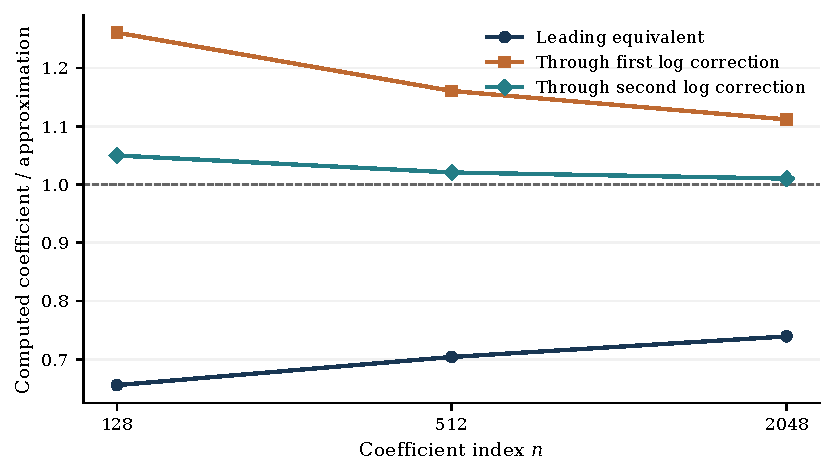
\includegraphics[width=0.83\textwidth]{figures/marginal_refinement.pdf}
\caption{The order-three coefficient divided by successive
asymptotic approximations.  Points are exact finite recurrences in
floating-point arithmetic; connecting segments only guide the eye.
The horizontal line is ratio one.  The three recorded indices are
$128$, $512$, and $2048$.}
\label{fig:marginal}
\end{figure}

For the inverse charts, a separate 180-digit program solves the
original polylogarithmic equation at $s=2.5,3,3.5,4$ and
$d=10^{-8},10^{-16},10^{-32}$.  The largest residual, divided by
$d$, is $1.89\cdot10^{-149}$ on this grid.  The same program verifies
the first core polynomials and the transferred logarithmic
corrections symbolically.  A 200-digit program independently checks
the critical order crossover for $\lambda=-2,0,2$ and $X=20,40,80$.
It evaluates both the original square-root deficit and the paired
equation.  At $X=80$, the observed relative errors after the second
algebraic correction range from $2.86\cdot10^{-6}$ to
$7.12\cdot10^{-5}$.  It also tests the exact first exponential
coefficient in \eqref{oc:first-exp-coefficient} against the difference
between the full solution and the complete algebraic core.
The separate joint-crossover program additionally tests nonzero
$\eta$, checks the selected real branch against the interior fold,
and includes a local complex-fold diagnostic; its complete parameters
and residuals are in \path{data/joint_crossover_checks.json}.
On the $18$-point joint grid, the maximum absolute relative error
of the first-corrected approximation decreases from $8.03\cdot10^{-3}$
at $X=40$ to $2.15\cdot10^{-3}$ at $X=80$.  All six negative-$\eta$
cases pass the independent fold-side check.  At the complex test
$k=1,X=40$, the full fold equations have tiny numerical residuals,
but the leading limiting constants still differ from the computed
$\alpha_c$ and $\omega_c$ by approximately $1.52$ and $0.317$,
respectively.  Solving the full equations accurately does not make
their leading asymptotic approximation equally accurate.

\begin{figure}[htbp]
\centering
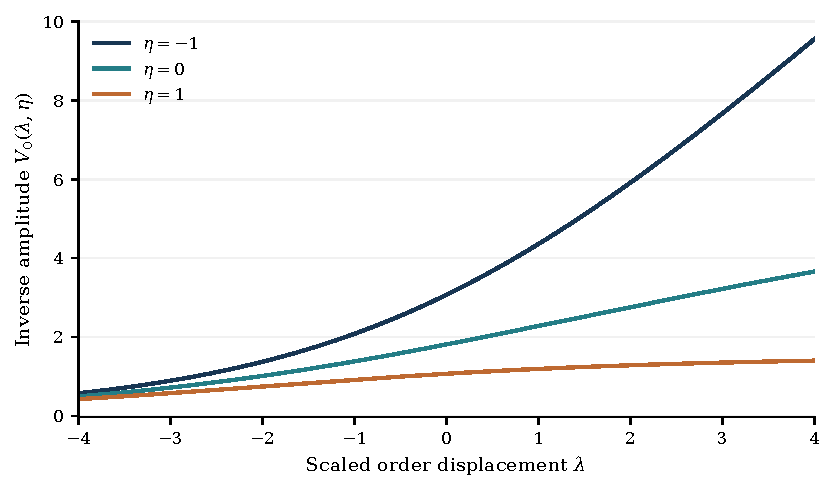
\includegraphics[width=0.87\textwidth]{figures/joint_profile.pdf}
\caption{The explicit positive profile $V_0(\lambda,\eta)$ in
\eqref{oc:profile}.  The curves are exact evaluations of the limiting
formula, not fitted numerical data.  They show how the order and
feedback displacements jointly determine the inverse amplitude.}
\label{fig:joint-profile}
\end{figure}

Finally, the coefficient-crossover program tests all $27$ combinations
of $s=2.5,3,4$, $n=128,512,2048$, and prescribed
$\xi=-1,0,1$.  The parameter $b$ is selected on the locally unique
branch near $A$, within $[A/2,2A]$.  This qualification matters:
for $s>3$ the map $b\mapsto\xi$ is not globally one-to-one on
$(0,\infty)$.  The stable density convention is independently checked
by 75-digit Fourier integration at $\xi=\pm1$ and by
\eqref{eq:stable-zero} at zero.  The largest relative difference from
the density evaluator is $5.15\cdot10^{-16}$.

\begin{figure}[htbp]
\centering
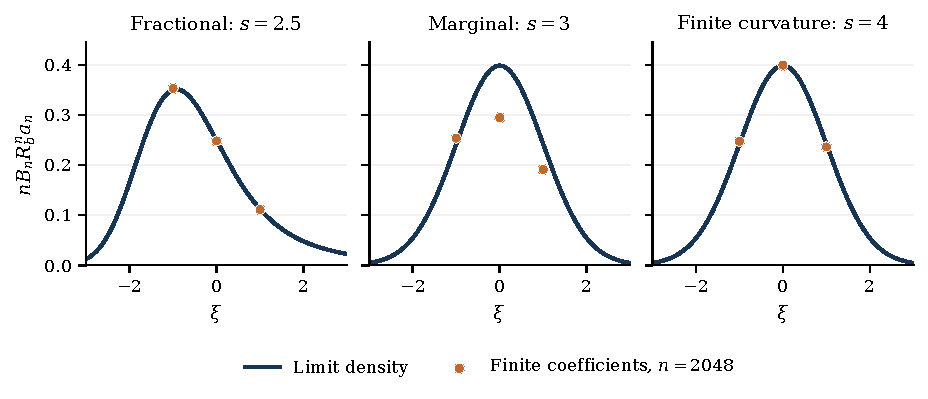
\includegraphics[width=\textwidth]{figures/coefficient_crossover.pdf}
\caption{Coefficient crossover in the normalization
$nB_n\Rb^n a_n$.  Curves are the stable or Gaussian limit densities;
points are the finite coefficient computation at $n=2048$ and
$\xi=-1,0,1$.  The elementary order-three normalization still has
visible logarithmic error.  Convergence need not be monotone at
every noncentral $\xi$.}
\label{fig:coefficient-crossover}
\end{figure}

\FloatBarrier
\subsection{What should change in the inspected material}

The source theorem for an interior characteristic point is correct in
its stated range.  Its boundary discussion was explicitly a proposed
research problem, so the missing proof should not be described as an
error.  The natural source update is to mark its supercritical
candidate as proved by \cref{thm:phase}, and replace its remaining
critical-endpoint question by the three exact laws
\eqref{eq:critical-stable}--\eqref{eq:critical-gaussian}.  The physical
convergence statement can then be extended from $0<s\le2$ to every
$s>0$ by \cref{cor:physical}.

The focused audit did not confirm a new false theorem in the inspected
incoming reports.  Several distinctions nevertheless need to survive
integration, because omitting them would create incorrect extensions:

\begin{enumerate}
\item \textbf{The endpoint reference is not always the Taylor radius.}
For $s>2$ and $b>0$, the equality $R=\Rb$ holds at and above the feedback threshold.
Below it, the physical germ first reaches an interior fold, whose
radius is larger than the endpoint reference.  The exact probability
identity still uses $\Rb$ on both sides.

\item \textbf{Integer orders require the paired expression.}
Gamma and zeta poles in the noninteger expansion cancel before any
integer limit.  For example the order-four term uses $H_3=11/6$,
not a separate value of $\zeta(1)$.  Similarly, the order-three
constant $5/2$ includes the quadratic feedback contribution.

\item \textbf{A function chart and a coefficient expansion have
different convergence claims.}
The charts in \cref{sec:charts,sec:order-crossover} are convergent
holomorphic substitutions.  The Gamma-derivative transfer series is
used only to a fixed asymptotic order.

\item \textbf{Local complex folds need a sheet qualification.}
\Cref{thm:local-complex-fold} describes continued local normal-form
solutions.  It does not locate a singularity of the original Taylor
germ without a separate global continuation argument.

\item \textbf{Uniformity requires stated parameter sets.}
In the lattice limit, $b$ stays in a compact positive interval.
The compact $\xi$ consequence then forces $b\to A$.  The theorem
does not cover an unrelated sequence $b\to0$, nor does an absolute
local-limit error prove a relative tail estimate in an expanding
$\xi$ window.
\end{enumerate}

The integration notes provide the source locations and a proposed
cross-reference paragraph.  They preserve the incoming source's
historical theorem labels and credit the earlier linear-tail models.
No existing theorem needs to be silently relabeled or removed.

\subsection{Further research questions and concrete targets}

The following questions are deliberately more specific than requests
for ``higher-order terms.''  Each identifies an additional statement
that is not proved by the present theorems.

\begin{enumerate}[label=\textbf{Q\arabic*.},leftmargin=2.7em]
\item \textbf{Joint coefficient asymptotics as both the order and
feedback vary.}
\Cref{thm:joint-crossover} treats the local inverse with varying
order; \cref{thm:coefficient-crossover} keeps the order fixed.
A natural next theorem would make the coefficient statement uniform
when
\[
 s_n=3+\eps_n,\qquad
 \lambda_n=\frac{\eps_n\log n}{2}
\]
stays bounded.  Pole pairing suggests the candidate scale
\[
 \widetilde B_n^2=\frac{n\log n}{2b_n}\ph(\lambda_n),
 \qquad
 \frac{n(1-\zeta(s_n-1)/b_n)}{\widetilde B_n}=O(1),
\]
and a Gaussian limit in this normalization.  This is a proposed
target, not a theorem claimed here.  The principal tasks are uniform
Fourier domination through the colliding poles, the first correction,
and comparison with the exact Lambert scale at $\lambda=0$.
The corresponding linear-tail results in \cite{RepoGaussian} are a
starting point, not a substitute for the nonlinear estimates.

\item \textbf{Relative matching in expanding crossover windows.}
Determine the largest positive and negative ranges of $\xi_n$ in
which a relative version of \eqref{eq:crossover-coefficient} holds.
On the positive side it should match the fixed supercritical
$n^{-s}$ law; on the negative side it should match the interior-fold
exponential factor.  Such a result requires a uniform large-deviation
or saddle analysis beyond the absolute local limit.

\item \textbf{Quantitative convergence radii for the charts.}
The holomorphic implicit function theorem supplies positive radii
uniformly on compact parameter sets, but not optimal computable ones.
Find certified polydiscs for the low-order, Lambert, and joint charts,
and rigorous truncation constants that can be used numerically.
The coefficient functions' possible pole at $w=2$ is an algebraic
clue; it is not already a determination of the chart's global boundary.

\item \textbf{Global access to the complex fold curves.}
For fixed nonzero $k$, decide which paths in the complex order and
feedback variables carry the original germ to the local branches of
\cref{thm:local-complex-fold}.  Determine their monodromy and whether
they ever become dominant singularities of a specified continuation.
The local two-sheet normal form alone cannot answer this question.

\item \textbf{All coefficient corrections away from the marginal
order.}
Transfer the exact charts into finite formulas for every correction
in the stable range and at higher orders, including cancellations
when different chart monomials produce the same power.  At rational
orders, distinguish merging exponents from zeros of reciprocal Gamma
factors.  The conditional disappearance of the ladder at
$\zeta(s-2)=-1$ gives a particularly clean test case.

\item \textbf{General analytic feedback potentials.}
Replace $uv-v^2/2$ by an analytic $F(v)$ with $F(0)=0$ and study
$F(v)=\Li_s(r\ee^v)$.  For $s>3$, if $F(v_b)=\zeta(s)$ and
$F'(v_b)=\zeta(s-1)$, the finite-curvature term is governed by
$\zeta(s-2)-F''(v_b)$.  Find hypotheses preserving positive
coefficients and global dominance, and classify what happens when
this curvature is tuned to zero.  The latter can create a higher
degeneracy and needs a different chart.

\item \textbf{Logarithmically weighted and slowly varying tails.}
Replace $k^{-s}$ by $k^{-s}(\log k)^q$, or by
$k^{-s}L(k)$ under explicit regularity assumptions.  Order derivatives
of the polylogarithm give exact finite logarithmic weights, linking
this problem to the incoming order-jet articles.  Determine which
tails still admit convergent finite-generator charts and which yield
only asymptotic scales.  A regular-variation equivalent alone cannot
imply an analytic convergent chart.

\item \textbf{Arithmetic support and several dominant points.}
The uniqueness proof uses the positivity of every coefficient.
For feedback supported on a proper lattice, classify the competing
root-of-unity singularities and the resulting periodic coefficient
laws.  More generally, identify the least support hypotheses under
which the strict triangle argument and aperiodic local limit remain
valid.

\item \textbf{Finite action cutoffs in the nonlinear kernel.}
Study truncations before and after the nonlinear transformation
$f_u(t)=u-\sqrt{u^2-2\Li_s(t)}$.  These are different operations.
Determine the cutoff required to preserve each critical coefficient
law and the crossover profile, and whether the prefix cancellations
in the linear endpoint literature survive the quadratic feedback.

\item \textbf{Certified and formal verification.}
Convert the finite coefficient recursions and Lagrange extraction
identities into proof-assistant statements first.  An interval
implementation of the sector bounds and Rouch\'e circles could then
certify explicit numerical domains.  Formalizing the global
continuation and logarithmic transfer steps is a separate, larger
project; the supplied numerical scripts do not accomplish it.
\end{enumerate}

Questions Q1--Q3 offer the most direct continuation of the present
analysis.  Q4 and Q6 address genuinely additional analytic structure;
Q7--Q9 connect the exact model to broader tail classes and the action
budgets already studied in the repository.  The existing finite
identities, positivity argument, and pole-paired normal form provide
concrete starting points for each direction.

\subsection{Reproducibility and integration}

The archive contains the master \path{article.tex}, its seven section
files, the bibliography source, the compiled PDF, five verification
programs, a figure-generation program, machine-readable records,
and integration notes.  The recorded data permit the figures and PDF
to be rebuilt without rerunning high-precision roots.  The optional
verification target recomputes all numerical and symbolic checks.
The README gives the commands, dependency versions, and a distinction
between exact arithmetic checks and numerical diagnostics.
The source provenance pins the repository revision and hashes the
specific comparison files and incoming archives.

\clearpage
\begin{thebibliography}{99}
\addcontentsline{toc}{section}{References}

\bibitem{RepoFeedback}
\emph{Resonant Polylogarithm Transseries: Gamma Borel Kernels,
Cyclotomic Order Jets, and Sharp Dilogarithm Reversion}.
Research draft prepared for Vladimir Reshetnikov, 11 October 2026.
ProveIt, \path{docs/incoming/Resonant_Polylogarithm_Transseries.zip},
inner file \path{Resonant_Polylogarithm_Transseries/article.tex}.
Theorem \texttt{thm:feedback} and first question in
Section \texttt{sec:future}. All repository sources below use the
snapshot in \cref{sec:scope}:
\url{https://github.com/VladimirReshetnikov/ProveIt/tree/6207c3d40047fd8d1400a4d509fee71c9a3a8132}.

\bibitem{RepoHahn}
\emph{Beyond Finite-Action Folds: Critical Hahn Transseries,
Stable Sector Asymptotics, and Sharp Action Budgets}.
Research draft prepared for Vladimir Reshetnikov, 29 September 2026.
ProveIt, \path{Analysis/Transseries/docs/series-and-transseries/Critical_Hahn_Transseries_Beyond_Finite_Action_Folds/article.tex}.
In particular Proposition \texttt{prop:exact}, Theorem
\texttt{thm:phases}, and Proposition \texttt{prop:local-crossover}.

\bibitem{RepoGaussian}
\emph{Through the Stable--Gaussian Endpoint: Uniform Critical
Transseries, Prefix-Independent Cutoff Corrections, and Conditional
Extremes}. Research article prepared for Vladimir Reshetnikov,
29 September 2026.
ProveIt, \path{Analysis/Transseries/docs/series-and-transseries/Stable_Gaussian_Endpoint_Uniform_Critical_Transseries/article.tex}.

\bibitem{RepoJets}
\emph{Polylogarithm Order Jets and Resonant Inversion}.
Research report, 12 October 2026.
ProveIt, \path{docs/incoming/polylogarithm_transseries_research.zip},
inner file \path{Polylogarithm_Order_Jets_2026-10-12/polylogarithm_order_jets.tex}.

\bibitem{RepoUniform}
\emph{Resonant Order Jets and Convergent Inverse Transseries for
Polylogarithms and Logarithmically Weighted Tails}.
Research draft prepared for Vladimir Reshetnikov, 12 October 2026.
ProveIt, \path{docs/incoming/polylogarithm_resonance_and_inverse_transseries.zip},
inner file \path{polylogarithm_resonance_and_inverse_transseries/polylogarithm_resonance_and_inverse_transseries.tex}.

\bibitem{RepoNormalized}
\emph{Resonant Polylogarithmic Jets and Convergent Inverse Transseries}.
Research contribution prepared for Vladimir Reshetnikov, 11 October 2026.
ProveIt, \path{docs/incoming/ProveIt_Resonant_Polylog_Transseries.zip},
inner file \path{ProveIt_Resonant_Polylog_Transseries/resonant_polylog_transseries.tex}.

\bibitem{RepoFolds}
\emph{Resonant Polylogarithm Inversion: Uniform Order Crossover,
Gamma--Zeta Fold Loci, and Convergent Exponential Sectors}.
Research contribution prepared for Vladimir Reshetnikov,
11 October 2026.
ProveIt, \path{docs/incoming/ProveIt_Resonant_Polylogarithm_Inversion_2026-10-11.zip},
inner file \path{resonant-polylogarithm-inversion/article.tex}.

\bibitem{DLMFPolylog}
NIST Digital Library of Mathematical Functions, \S25.12,
\emph{Polylogarithms}, especially Eq.~25.12.12.
\url{https://dlmf.nist.gov/25.12}.
Accessed 12 October 2026.

\bibitem{DLMFLambert}
NIST Digital Library of Mathematical Functions, \S4.13,
\emph{Lambert $W$-Function}.
\url{https://dlmf.nist.gov/4.13}.
Accessed 12 October 2026.

\bibitem{FO}
P.~Flajolet and A.~Odlyzko,
\emph{Singularity analysis of generating functions},
SIAM Journal on Discrete Mathematics \textbf{3} (1990), 216--240.
\href{https://doi.org/10.1137/0403019}{doi:10.1137/0403019}.
Author-hosted text:
\url{https://algo.inria.fr/flajolet/Publications/FlOd90b.pdf}.

\bibitem{Janson}
S.~Janson,
\emph{Simply generated trees, conditioned Galton--Watson trees,
random allocations and condensation},
Probability Surveys \textbf{9} (2012), 103--252.
\href{https://doi.org/10.1214/11-PS188}{doi:10.1214/11-PS188}.
\url{https://arxiv.org/abs/1112.0510}.

\end{thebibliography}

\end{document}
